\documentclass[preprint,12pt,authoryear]{elsarticle}

%% Use the option review to obtain double line spacing
%% \documentclass[authoryear,preprint,review,12pt]{elsarticle}

\usepackage{booktabs}
\usepackage{tabularx}
\usepackage{array}
\usepackage{caption}
\captionsetup[table]{skip=8pt}
\usepackage{microtype}
\emergencystretch=1em

\providecommand{\code}[1]{\texttt{#1}}

%% The amssymb package provides various useful mathematical symbols
\usepackage{amssymb}
%% The amsmath package provides various useful equation environments.
\usepackage{amsmath}
%% The amsthm package provides extended theorem environments
%% \usepackage{amsthm}

%% The lineno packages adds line numbers. Start line numbering with
%% \begin{linenumbers}, end it with \end{linenumbers}. Or switch it on
%% for the whole article with \linenumbers.
%% \usepackage{lineno}
\usepackage[colorlinks=true,allcolors=blue]{hyperref}

\journal{\textcolor{blue}{Expert Systems with Applications}}

\usepackage{tikz}
\usetikzlibrary{positioning}
\usepackage{float}
\usepackage{graphicx}

\begin{document}

\begin{frontmatter}

\title{\textcolor{blue}{TrustStatAgent: Conformally calibrated release decisions for large language model statistical agents}}

\author{} %% Author name

%% Author affiliation
\affiliation{organization={},%Department and Organization
            addressline={}, 
            city={},
            postcode={}, 
            state={},
            country={}}

%% Abstract
\begin{abstract}
Delegating statistical analysis to large language model (LLM) agents is attractive because the work is repetitive and tool-heavy, but an erroneous result is consumed downstream as a fact. Existing pipelines leave the release decision to the user or to a confidence threshold tuned once on validation data, which carries no finite-sample guarantee and, on the forecasting task, is outperformed by publishing everything. To address these limitations, this paper presents TrustStatAgent: a tool-restricted LLM plans the analysis and routes every computation through statistical tools; conformal calibration turns each candidate into an interval or label set with finite-sample coverage; and a deterministic gate releases a result only when its execution checks pass and the calibrated output lies inside the task's acceptance region, referring the rest to human review. The model that produces a number never decides whether that number is published, and every referred result carries the condition it failed. On four benchmarks covering question answering, classification, regression and forecasting, the gate attains the lowest released error rate, reducing it from 27.16\% to 1.87\% on StatQA at a 46.12\% release rate and from 15.33\% to 2.72\% on Adult at 54.29\%, with base accuracy retained at 72.84\% and 84.67\%. The gain is not free: between 22.28\% and 53.88\% of results are referred for review, and forecasting automation falls by 10.4 percentage points against conventional gating. The release rate accompanies every reliability figure, so an operator can weigh the exchange against the ratio of the cost of a published violation to a referral.
\end{abstract}

%%Graphical abstract
\begin{graphicalabstract}
\textcolor{blue}{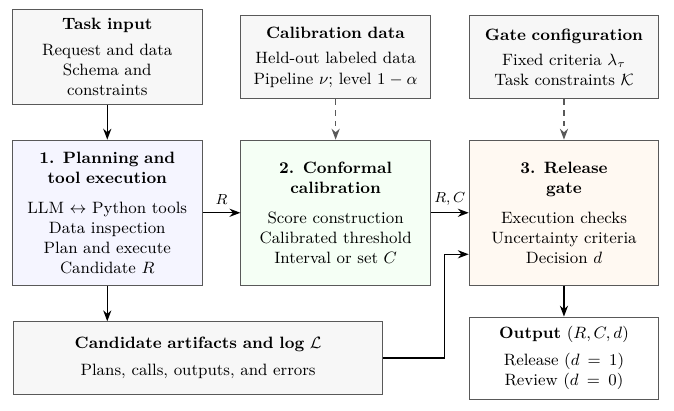
\includegraphics[width=\linewidth]{figures/download.png}}
\end{graphicalabstract}

%%Research highlights
\begin{highlights}
\item \textcolor{blue}{A statistical agent that separates result generation from result release}
\item \textcolor{blue}{Conformal calibration attaches finite-sample coverage to each result}
\item \textcolor{blue}{A deterministic gate releases only results inside acceptance regions}
\item \textcolor{blue}{Released error falls from 27.16\% to 1.87\% on StatQA at 46.12\% release}
\item \textcolor{blue}{On Carbon Monitor, conventional gating intercepts no error at all}
\end{highlights}

%% Keywords
\begin{keyword}
{\color{blue}
Large language model agents \sep Conformal prediction \sep Selective prediction \sep Uncertainty quantification \sep Statistical analysis \sep Risk control
}
\end{keyword}

\end{frontmatter}

\section{Introduction}
\label{sec1}



Large language models (LLMs) are increasingly deployed as the reasoning core of expert systems. This shift rests on two capabilities. The first is reasoning: chain-of-thought prompting decomposes a difficult problem into intermediate steps and markedly improves arithmetic and symbolic inference~\citep{wei2022chain}, a behaviour that can be triggered without demonstrations~\citep{kojima2022large} and stabilised by sampling and voting~\citep{wang2023self}. The second is acting: ReAct interleaves reasoning traces with calls to external tools~\citep{yao2023react}, and Toolformer shows that the decision of when to invoke an interface can be learned~\citep{schick2023toolformer}.

Statistical analysis is among the domains in which this capability matters most, because the work involved, such as fitting models, selecting estimators and reporting intervals, is repetitive and tool-heavy. Interest in delegating such work to LLM-based data agents has therefore grown rapidly~\citep{sun2026survey}. Systematic evaluation nevertheless indicates that the capability gap remains wide. On StatQA, a benchmark of 11{,}623 statistical-analysis items, the strongest model attains only 64.83\% accuracy, and its errors are dominated by method applicability rather than computation~\citep{zhu2024large}. The bottleneck is therefore not arithmetic, which can be delegated to deterministic tools, but the judgement surrounding it.

That judgement is also where the reliability of LLMs is weakest. LLMs generate content unfaithful to the available evidence~\citep{ji2023survey}, and their confidence signals are poorly calibrated~\citep{guo2017calibration,kadavath2022language}. Within a statistical pipeline such failures are not merely textual. A misspecified model or an interval that does not cover the quantity it claims to cover is consumed downstream as a fact, and the error is silent. An autonomous statistical agent must therefore decide, for each result, whether that result is safe to release.

Making this requirement precise exposes a difficulty. If reliability is measured as the proportion of released results that are correct, an agent that releases nothing attains a perfect score while completing none of the workload. Reliability is therefore informative only when reported jointly with the fraction of tasks the agent publishes. The objective adopted here is accordingly the joint attainment of statistical accuracy and publishing reliability, which raises three questions. Can a tool-restricted agent match uncalibrated baselines on heterogeneous tasks? Can conformal prediction convert its heuristic uncertainty into statements with finite-sample validity? And does a calibrated gate discriminate publishable from non-publishable results better than a threshold tuned once on validation data?

An uncertainty layer is the first requirement. Confidence scores are model-specific and carry no finite-sample statement about the quantity of interest. Conformal prediction provides one: it is model-agnostic and distribution-free, and it constructs prediction sets with non-asymptotic coverage guarantees that remain valid under a misspecified model~\citep{lei2018distribution,angelopoulos2021gentle}, with recent extensions controlling the expectation of arbitrary monotone losses~\citep{angelopoulos2024conformal}. Conformal methods have accordingly reached natural language processing~\citep{campos2024conformal,wang2024conu,cherian2024large}. What remains missing is their coupling to the execution of the analysis.

A second requirement concerns how uncertainty becomes an action. Selective prediction formalises the trade-off between coverage and risk and allows a model to abstain where a target risk cannot be met~\citep{geifman2017selective}. In conventional deployments, including the baseline used here, the rejection threshold is tuned once on a validation set and then frozen, which provides no guarantee on the test distribution. Deriving it instead from a quantile of calibration scores lets the decision rule inherit that guarantee. Reliability mechanisms for LLM agents have also attracted attention in the expert-systems community~\citep{shi2025mitigating,he2026enhancing}. The present work supplies a statistical guarantee rather than a consensus heuristic, and attaches it to the decision to publish.

To address these issues, this paper proposes TrustStatAgent, a statistical agent that combines three components. The first is an LLM acting as a planning brain: given a task specification and a restricted toolset for data inspection, model fitting and prediction, it identifies the target variable, the candidate inputs and the task type, emits a structured plan, and routes every numerical computation through the tools. Its instructions forbid fabricated results and forbid the model from deciding whether its own output may be released. The second is conformal calibration, which uses the $\lceil (n+1)(1-\alpha)\rceil$-th smallest nonconformity score on a held-out split to turn point forecasts into intervals and probabilistic label sets into prediction sets. The third is a risk gate, which publishes a result only when its conformal output is valid and a deterministic execution check passes, and defers all other cases to human review.

% ---------------------------------------------------------------------
% TODO —— 待补：实验发现（当前为占位，投稿前必须替换为正式内容）
%
% 计划写入第 5 节的三项发现：
%   (1) TrustStatAgent 与三个基线在基础统计任务上的表现对比（表 1）
%   (2) 常规验证集调参门控 vs 共形门控，在发布判别指标上的对比（表 2）
%   (3) 依次移除显式规划、共形校准、风险门控的消融实验（表 3）
%
% 补齐后取消下列 \iffalse ... \fi 的注释即可。
% ---------------------------------------------------------------------
\iffalse
% 实验发现段落占位，待补。
\fi

In summary, the main contributions of this paper are as follows:
\begin{itemize}
  \item We formulate the deployment of LLM-based statistical agents as a joint objective of statistical accuracy and publishing reliability, and we make explicit the evaluation trap whereby a reliability-only criterion can be satisfied through excessive abstention.
  \item We propose TrustStatAgent, which couples tool-grounded execution checking with conformally calibrated uncertainty and a conformal risk gate within a single workflow, separating result generation from result release at the architectural level.
  \item We replace the validation-tuned rejection threshold with a conformally calibrated gate, and compare the two directly in their ability to discriminate publishable from non-publishable results.
  \item We evaluate the framework on four heterogeneous statistical tasks, namely regression on California Housing~\citep{pace1997sparse}, binary classification on UCI Adult~\citep{becker1996adult}, time-series forecasting on Carbon Monitor~\citep{liu2020carbon} and statistical question answering on StatQA~\citep{zhu2024large}, and we isolate the contribution of explicit planning, conformal calibration and risk gating through targeted ablations.
\end{itemize}

%This paper is organized as follows. Section~2 reviews related work on LLM agents, uncertainty quantification and selective prediction. Section~3 presents the TrustStatAgent framework. Section~4 describes the datasets, baselines and evaluation metrics. Section~5 reports and discusses the experimental results. Section~6 concludes the paper and outlines directions for future work.

\section{Related Work}
\subsection{Large language model agents for statistical analysis}
\label{subsec:statistical_agents}
Large language models (LLMs) offer a new interface for data analysis through natural language. Users can describe an analytical task, and the model can identify relevant variables, organize the required steps,and invoke external tools to perform computations. In this workflow, the LLM interprets the task and plans the analysis, while statistical tools perform numerical computations and execute models. ReAct interleaves reasoning and actions so that models can adjust their task trajectories using external feedback~\citep{yao2023react}.Data Interpreter extends this approach to multistage data analysis by representing task dependencies as a graph and incorporating iterative verification and correction~\citep{hong2025data}.These studies provide a foundation for translating natural language requests into executable workflows.

Statistical analysis imposes explicit constraints on variable definitions, data types, and the applicability of methods. Consequently, a computation that returns successfully does not establish that the analytical choices were appropriate. StatQA evaluates the joint selection of relevant variables and applicable statistical methods and identifies limitations in LLMs' assessment of method applicability~\citep{zhu2024large}. Evaluating a statistical agent therefore requires distinguishing task interpretation, method selection, and tool execution. 

Existing research on tool use provides mechanisms for generating candidate statistical results. Whether these results are suitable for direct use, however, requires further assessment. Conformal inference provides a principled way to supplement point predictions with prediction intervals offering finite-sample marginal coverage under exchangeability~\citep{lei2018distribution}. Methodological choices also warrant scrutiny: independent teams analyzing the same dataset can obtain substantially different results through different analytical workflows~\citep{botvinik2020variability}. Furthermore, selective classification explicitly distinguishes prediction from the decision to accept or reject it, formalizing the trade-off between predictive risk and the proportion of accepted predictions~\citep{elyaniv2010foundations}. Motivated by these considerations, we introduce uncertainty calibration and release decisions as separate stages after tool execution. This design connects task execution with result release and retains the variables, methods, and execution records used to produce each candidate, providing evidence for subsequent decisions.

\subsection{Statistical uncertainty and conformal prediction}
\label{subsec:uncertainty_conformal}
Uncertainty quantification helps connect model predictions with practical decisions. Probabilistic modeling provides a basis for representing and handling uncertainty in models and predictions~\citep{ghahramani2015probabilistic}. For statistical agents, a point prediction or a single candidate answer provides limited information about the strength of the supporting evidence. Moreover, uncalibrated model probabilities may not accurately reflect predictive reliability.

Conformal prediction uses a separate calibration sample to construct prediction intervals or sets and provides finite-sample marginal coverage guarantees under appropriate exchangeability conditions~\citep{angelopoulos2021gentle}. Because conformal prediction can be applied around an existing predictor, it can accommodate outputs from different statistical tools. For regression, conformalized quantile regression (CQR) combines quantile predictions with conformal calibration to produce intervals that reflect variation in uncertainty across observations~\citep{romano2019cqr}. For classification, nonconformity scores can be constructed from the predicted probability of the true class, yielding sets containing one or more candidate classes.

\subsection{Output verification and selective release}
\label{subsec:verification_release}
Trustworthy artificial intelligence encompasses transparency, explainability, fairness, privacy, and reproducibility, among other dimensions. Each system must specify which dimensions it addresses within its intended task~\citep{li2023trustworthy}. Post-generation verification can provide an assessment of model outputs that is separate from the generation process. HaluCheck uses the AutoFactNLI pipeline to decompose generated content, retrieve external evidence, and assess factual relationships, while presenting users with traceable verification results~\citep{heo2025halucheck}. This work highlights the value of inspectable evidence in an evaluation layer: users need to assess whether an output meets predefined requirements alongside any statistical uncertainty representation.

Selective prediction allows a system to abstain on some inputs when the available evidence is insufficient, while considering both prediction risk and the acceptance rate. SelectiveNet integrates prediction with a reject option and examines the trade-off between risk and coverage~\citep{geifman2019selectivenet}. For language model outputs, conformal methods have been used to construct output sets, demonstrating how statistical calibration can contribute to reliability assessment~\citep{quach2024conformal}.

Building on these studies, TrustStatAgent is designed as a calibration and release workflow for heterogeneous statistical tasks. Authorized tools generate candidate results, calibration procedures tailored to the target produce prediction intervals or sets, and execution checks and task requirements determine whether each result can be released automatically.


\section{Methodology}
\label{sec:methodology}
This section describes TrustStatAgent, a workflow for deciding when statistical results can be released automatically. As illustrated in Fig.~\ref{fig:framework}, it combines LLM task planning and statistical tool execution, uncertainty calibration, and a risk gate. We first define the overall framework, then describe these three components in turn.

\subsection{Framework and task formulation}
\label{sec:framework}

TrustStatAgent separates task planning and statistical execution, uncertainty calibration, and result release. For a task specification $\mathcal{T}$ and authorized tools $\mathcal{F}$, the first module produces a statistical result $R$ and an execution record $\mathcal{L}$. Calibration then constructs an interval or set $C$ from held-out data, and a deterministic gate produces a release decision $g$:
\begin{equation}
    (R,\mathcal{L})=\mathcal{A}_{\theta}(\mathcal{T};\mathcal{F}),\qquad
    C=\mathcal{Q}_{\alpha}(R;\mathcal{D}_{\mathrm{cal}}),\qquad
    g=\mathcal{G}_{\tau}(R,C,\mathcal{L};\Omega),
    \label{eq:framework}
\end{equation}
where $\theta$ denotes the language-model configuration, $\tau$ is the task type, $\alpha$ is the nominal miscoverage level, and $\Omega$ contains task-specific acceptance criteria. The LLM interprets the request and specifies the analysis; authorized programs perform numerical computation and retain execution evidence. A result is released only when its calibrated output and execution status meet the prespecified criteria. We evaluate this design on three predictive tasks and one structured statistical question-answering task, with task-specific implementations described below.

\begin{figure}[!htbp]
    \centering
    % Replace the filename and uncomment this line after adding your image.
    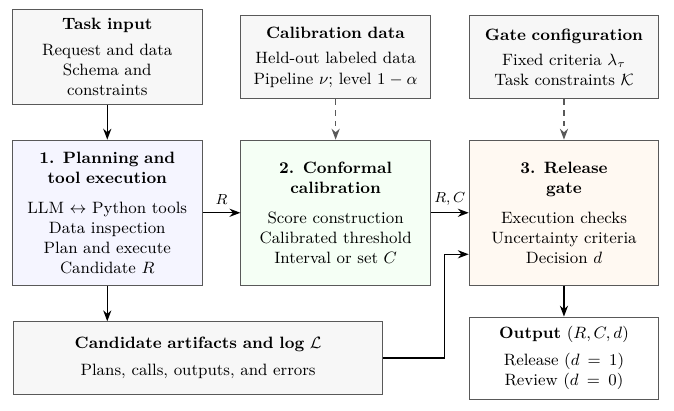
\includegraphics[width=\linewidth]{figures/download.png}
    \caption{Overall architecture of TrustStatAgent.
    Solid arrows denote task information, candidate results, or execution evidence; dashed arrows denote calibration resources and release configurations.
    Statistical computation, calibration, and gating are performed by programs.
    Unresolved execution failures or unavailable conformal outputs lead to human review.
    Calibration labels remain outside the LLM interaction, and test labels are used only for evaluation.}
    \label{fig:framework}
\end{figure}

\subsection{Task planning and statistical tool execution}
\label{sec:execution}

The first module translates a natural-language request into an executable analysis. Following the reasoning-and-action pattern of ReAct~\citep{yao2023react}, the LLM receives the user's request, descriptions of the available datasets, and specifications of the permitted statistical tools. It records a structured plan containing the task type, target, selected variables, method, preprocessing, and intended tool sequence. Explicit variable and method selection addresses a documented difficulty in statistical question answering~\citep{zhu2024large}. For numerical tasks, the LLM selects tools for data inspection, model fitting, prediction, or forecasting. Each requested tool call is checked against the permitted tool set and executed by the corresponding statistical procedure. The results are recorded and returned to the LLM to guide subsequent analysis.

For each predictive task, the model configuration and preprocessing procedures are kept fixed across experimental variants to ensure reproducible evaluation. California Housing uses gradient-boosting models for point and quantile predictions, Adult uses a logistic-regression pipeline, and Carbon Monitor uses a seasonal-naive forecast. In StatQA, the LLM returns the selected columns and methods under an explicit plan, and the benchmark evaluates these analytical choices directly. Its answer correctness follows the benchmark criterion~\citep{zhu2024large}, while a separate TF--IDF logistic-regression scorer supplies the score used for calibration. The scorer is trained on a dedicated split, and reference answers are excluded from its input features.
Figure~\ref{fig:planning_execution} illustrates this
workflow using a house-value prediction request.

\begin{figure}[!htbp]
    \centering
    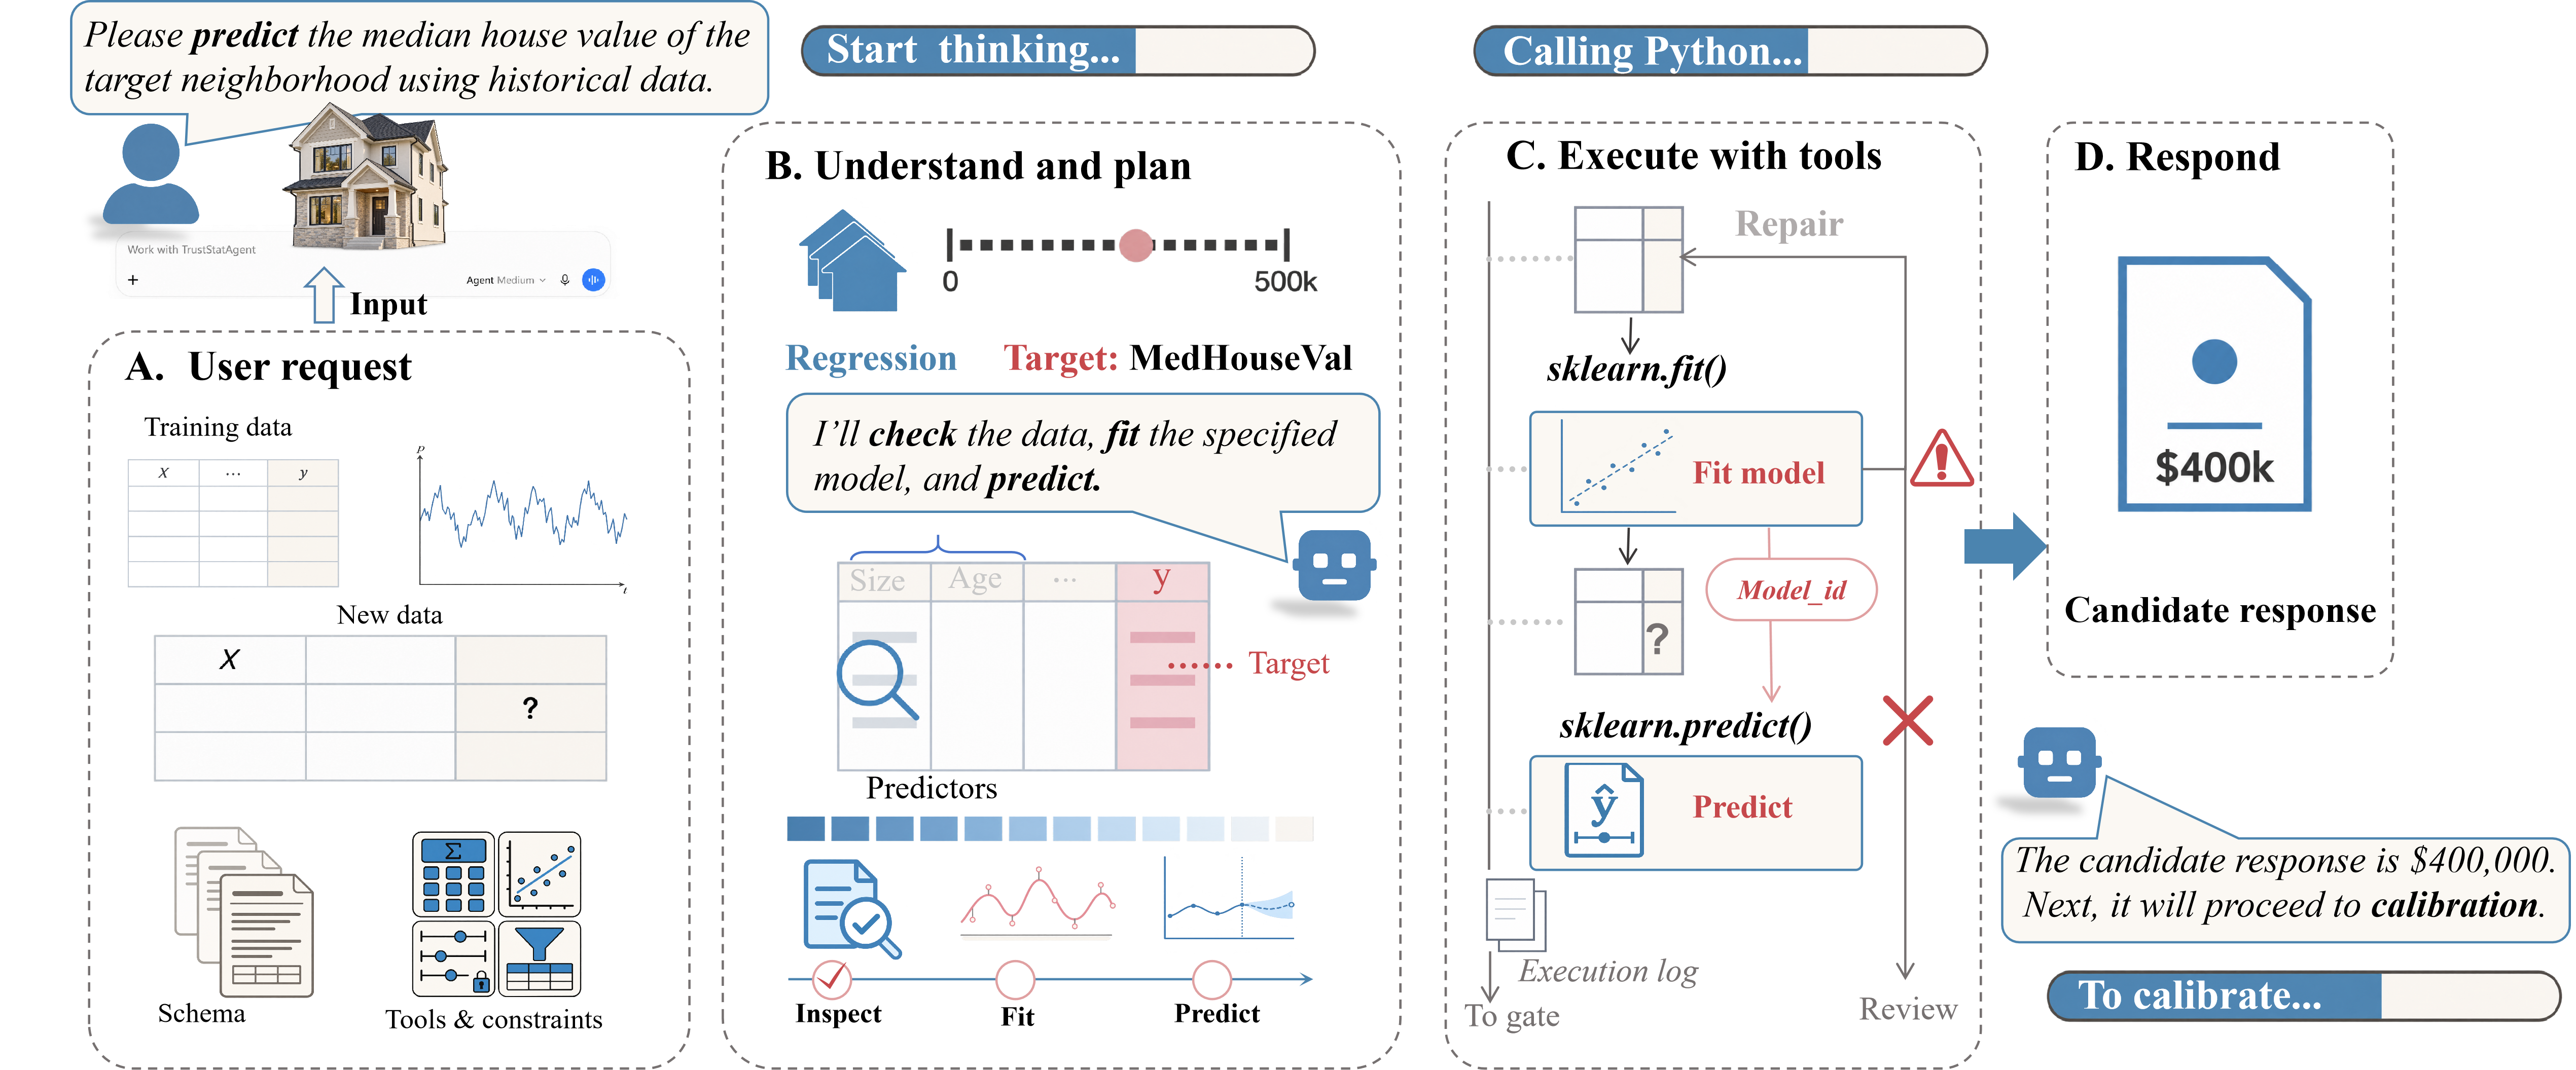
\includegraphics[width=\linewidth]{sci1.png}
    \caption{LLM task planning and statistical tool execution}
    \label{fig:planning_execution}
\end{figure}

\subsection{Conformal uncertainty calibration}
\label{sec:uncertainty_calibration}
For each candidate result, the calibration module constructs an interval or prediction set for the corresponding target using scores computed on calibration data. Following the
conformal prediction framework \citep{angelopoulos2023gentle}, the target
is the response value for regression and forecasting, the class label
for classification, and candidate correctness for statistical question
answering. The resulting intervals and prediction sets are evaluated against the release criteria defined in Section 3.4 to determine whether each candidate result can be released automatically.

Let \(R_i\) denote the candidate generated from observable inputs \(x_i\),
and let \(T_i\) denote its calibration target. A nonconformity score
\(s_\tau(x_i,R_i,T_i)\) measures their incompatibility for task type
\(\tau\), with larger values indicating greater incompatibility.
Predictors, preprocessing procedures, and correctness scorers are fitted
separately from the records used to calculate calibration scores.

For \(n\) calibration scores ordered as
\(s_{(1)}\leq\cdots\leq s_{(n)}\), the operational threshold at nominal
miscoverage level \(\alpha\) is
\begin{equation}
    k_\alpha
    =
    \left\lceil(n+1)(1-\alpha)\right\rceil,
    \qquad
    \widehat q_\alpha
    =
    s_{(\min\{k_\alpha,n\})}.
    \label{eq:calibration_threshold}
\end{equation}
The corresponding calibrated set is
\begin{equation}
    C_\alpha(x_i,R_i)
    =
    \left\{
        u\in\mathcal{Y}_\tau:
        s_\tau(x_i,R_i,u)\leq\widehat q_\alpha
    \right\},
    \label{eq:calibrated_target_set}
\end{equation}
where \(\mathcal{Y}_\tau\) is the target space. Scores and thresholds are calculated separately for each
task setting.
Figure~\ref{fig:conformal_calibration} summarizes the four
task-specific calibration procedures described below.

\begin{figure}[!htbp]
    \centering
    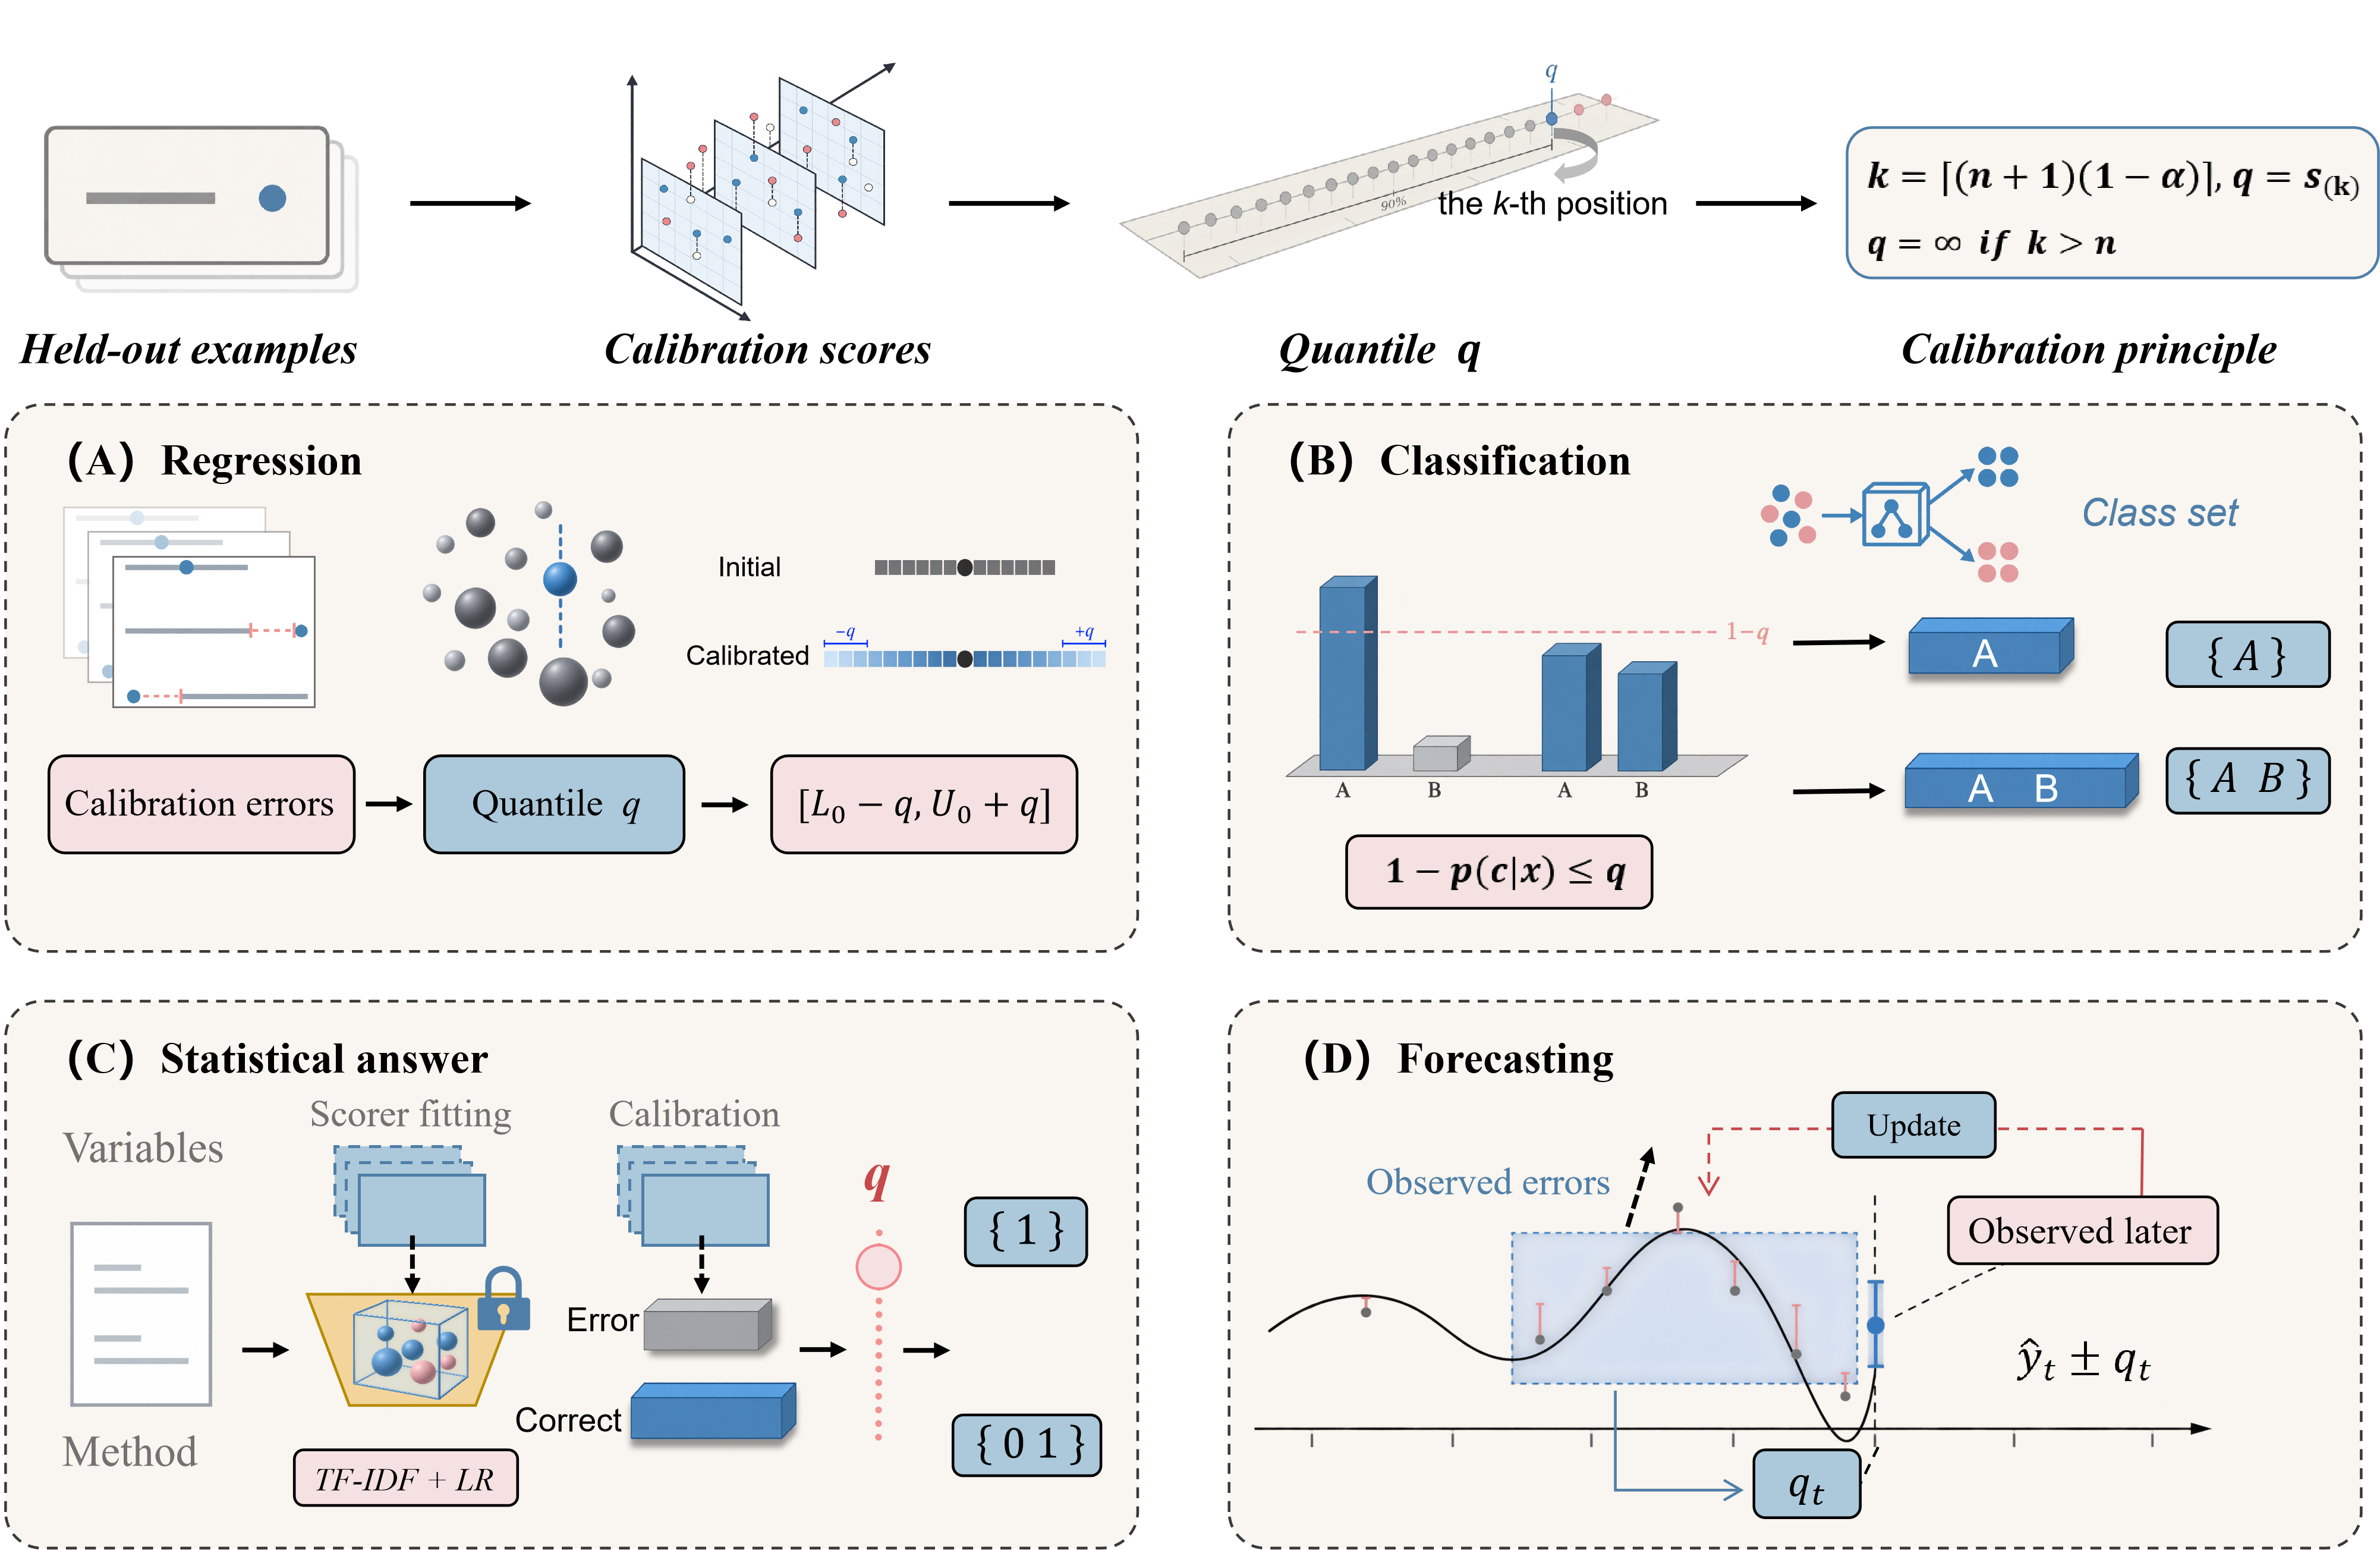
\includegraphics[width=\linewidth]{sci2.png}
    \caption{Task-specific conformal uncertainty calibration.}
    \label{fig:conformal_calibration}
\end{figure}

\begin{itemize}

    \item \textbf{Numerical prediction.}
    For California Housing, we use conformalized quantile regression
    \citep{romano2019cqr}. Given preliminary lower and upper quantile
    estimates \(L_0(x)\) and \(U_0(x)\), the calibration score is
    \begin{equation}
        s_i
        =
        \max\left\{
            L_0(x_i)-y_i,\;
            y_i-U_0(x_i)
        \right\}.
        \label{eq:cqr_nonconformity}
    \end{equation}
    With \(q^{+}=\max\{0,\widehat q_\alpha\}\), the calibrated interval is
    \begin{equation}
        C_i
        =
        \left[
            L_0(x_i)-q^{+},\;
            U_0(x_i)+q^{+}
        \right].
        \label{eq:cqr_calibrated_interval}
    \end{equation}
    The adjustment preserves variation in the preliminary interval
    widths across inputs, while the nonnegative correction prevents
    calibration from contracting the interval. The point prediction
    is retained separately for the subsequent tolerance-based
    release test.

    \item \textbf{Categorical prediction.}
    For Adult, the fitted classifier supplies class probabilities
    \(p(c\mid x_i)\). We use probability-threshold calibration
    \citep{angelopoulos2023gentle}, with scores
    \(s_i=1-p(y_i\mid x_i)\) and prediction sets
    \begin{equation}
        C_i
        =
        \left\{
            c:
            1-p(c\mid x_i)\leq\widehat q_\alpha
        \right\}.
        \label{eq:categorical_prediction_set}
    \end{equation}
    The resulting set may be empty, contain a single class, or retain
    multiple competing classes. It is passed to the gate together
    with the original predicted class, allowing release decisions
    to account for classification ambiguity.

    \item \textbf{Structured statistical answers.}
    Selective assessment requires an explicit criterion for output
    correctness \citep{lee2024selective}. For StatQA, let \(Z_i=1\)
    when the candidate's selected variables and statistical methods
    both match the reference sets under the benchmark's normalized
    exact-match criterion, and \(Z_i=0\) otherwise.

    A correctness scorer, trained on a separate scorer-training split
    and then frozen, produces \(r_i\in[0,1]\) from the observable task
    category and the generated selections. Calibration uses
    \begin{equation}
        s_i
        =
        Z_i(1-r_i)+(1-Z_i)r_i,
        \label{eq:statqa_nonconformity}
    \end{equation}
    yielding the correctness set
    \begin{equation}
        C_i
        =
        \left\{
            z\in\{0,1\}:
            z(1-r_i)+(1-z)r_i\leq\widehat q_\alpha
        \right\}.
        \label{eq:statqa_correctness_set}
    \end{equation}
    Reference answers supply offline training and calibration labels
    but are excluded from the scorer's inputs when assessing a new
    candidate. Thus, the calibrated target concerns the benchmark's
    structured analytical choices rather than unrestricted
    natural-language factuality.

    \item \textbf{Temporal prediction.}
    Online conformal methods explicitly address sequential calibration
    \citep{angelopoulos2024online}. For Carbon Monitor, we use a
    chronological rolling-residual construction around the lagged-value
    forecast specified by the task protocol. At time \(t\), let
    \(\mathcal{W}_t\) index the most recent \(w\) forecasts whose
    outcomes have already been observed. Their scores are
    \begin{equation}
        s_j
        =
        \left|y_j-\widehat y_j\right|,
        \qquad j\in\mathcal{W}_t.
        \label{eq:rolling_residual_scores}
    \end{equation}
    Applying Eq.~\eqref{eq:calibration_threshold} to these scores
    gives \(q_{\alpha,t}\) and the interval
    \begin{equation}
        C_t
        =
        \left[
            \widehat y_t-q_{\alpha,t},\;
            \widehat y_t+q_{\alpha,t}
        \right].
        \label{eq:rolling_calibrated_interval}
    \end{equation}
    Specifically, for Carbon Monitor, we use the previous observation as the forecast and construct the prediction interval from recent absolute prediction errors.

\end{itemize}



\subsection{Risk gating and selective release}
\label{sec:risk_gating}

The risk gate converts calibrated uncertainty into a decision about
automatic release. Recent work on informative conformal prediction examines how
prediction sets can be selected to meet application needs
\cite{gazin2025selecting}, while conformal risk control uses
specified loss functions to calibrate prediction rules
\cite{angelopoulos2024conformal}. In our framework, the
release criteria define which target values are acceptable.
A candidate is eligible for automatic release only if every
value or label in its calibrated set meets these criteria.

Let \(\mathcal{A}_{\Omega,i}\) denote the acceptable target set for
candidate \(i\), with requirements \(\Omega\) fixed before test
evaluation. Let \(H_i=1\) indicate an unresolved execution failure,
and let \(V_i=1\) indicate an available, valid uncertainty output.
Numerical intervals must have finite, ordered endpoints, while
discrete sets must be nonempty and contain admissible labels.
The release decision is
\begin{equation}
    g_i
    =
    \mathbf{1}\{H_i=0\}
    \mathbf{1}\{V_i=1\}
    \mathbf{1}\{C_i\subseteq\mathcal{A}_{\Omega,i}\},
    \label{eq:unified_release_gate}
\end{equation}
where \(g_i=1\) denotes automatic release and \(g_i=0\) denotes referral.
The validity condition excludes empty sets, whose mathematical
containment in any acceptance set would otherwise permit release
without supporting evidence.

For numerical predictions, the acceptable target set is
\begin{equation}
    \mathcal{A}_{\Omega,i}
    =
    \left[
        \widehat y_i-\Delta,\;
        \widehat y_i+\Delta
    \right],
    \label{eq:numerical_acceptance_set}
\end{equation}
where \(\Delta>0\) specifies the permitted prediction error.
Containment checks both interval endpoints relative to the point
prediction. For categorical
predictions, the acceptable set is the predicted-class singleton;
for StatQA, it is the correctness label \(\{1\}\).
Table~\ref{tab:calibrated_release_conditions} summarizes the
resulting conditions.

\begin{table}[t]
    \centering
    \caption{Automatic-release conditions. All conditions additionally
    require successful execution and a valid uncertainty output.}
    \label{tab:calibrated_release_conditions}
    \small
    \setlength{\tabcolsep}{3pt}
    \renewcommand{\arraystretch}{1.2}
    \begin{tabularx}{\columnwidth}{
        @{}
        >{\raggedright\arraybackslash}p{0.24\columnwidth}
        >{\raggedright\arraybackslash}p{0.25\columnwidth}
        >{\raggedright\arraybackslash}X
        @{}
    }
        \toprule
        Output type
        & Calibrated output
        & Release condition \\
        \midrule

        Regression
        & \([L_i,U_i]\)
        & \(L_i\geq\widehat y_i-\Delta\),\newline
          \(U_i\leq\widehat y_i+\Delta\) \\

        Classification
        & Class set \(C_i\)
        & \(C_i=\{\widehat y_i\}\) \\

        Statistical QA
        & Correctness set \(C_i\)
        & \(C_i=\{1\}\) \\

        Forecasting
        & \(\widehat y_t\pm q_{\alpha,t}\)
        & \(q_{\alpha,t}\leq\Delta\) \\

        \bottomrule
    \end{tabularx}
\end{table}

The gate automatically releases a candidate when execution
succeeds, the uncertainty output is valid, and the acceptance
criterion is satisfied. All remaining candidates are referred
for review. The gate makes the final release decision according
to these predefined rules.
Figure~\ref{fig:risk_gating} illustrates the checks,
acceptance tests, and routing decisions of the release gate.

\begin{figure}[!htbp]
    \centering
    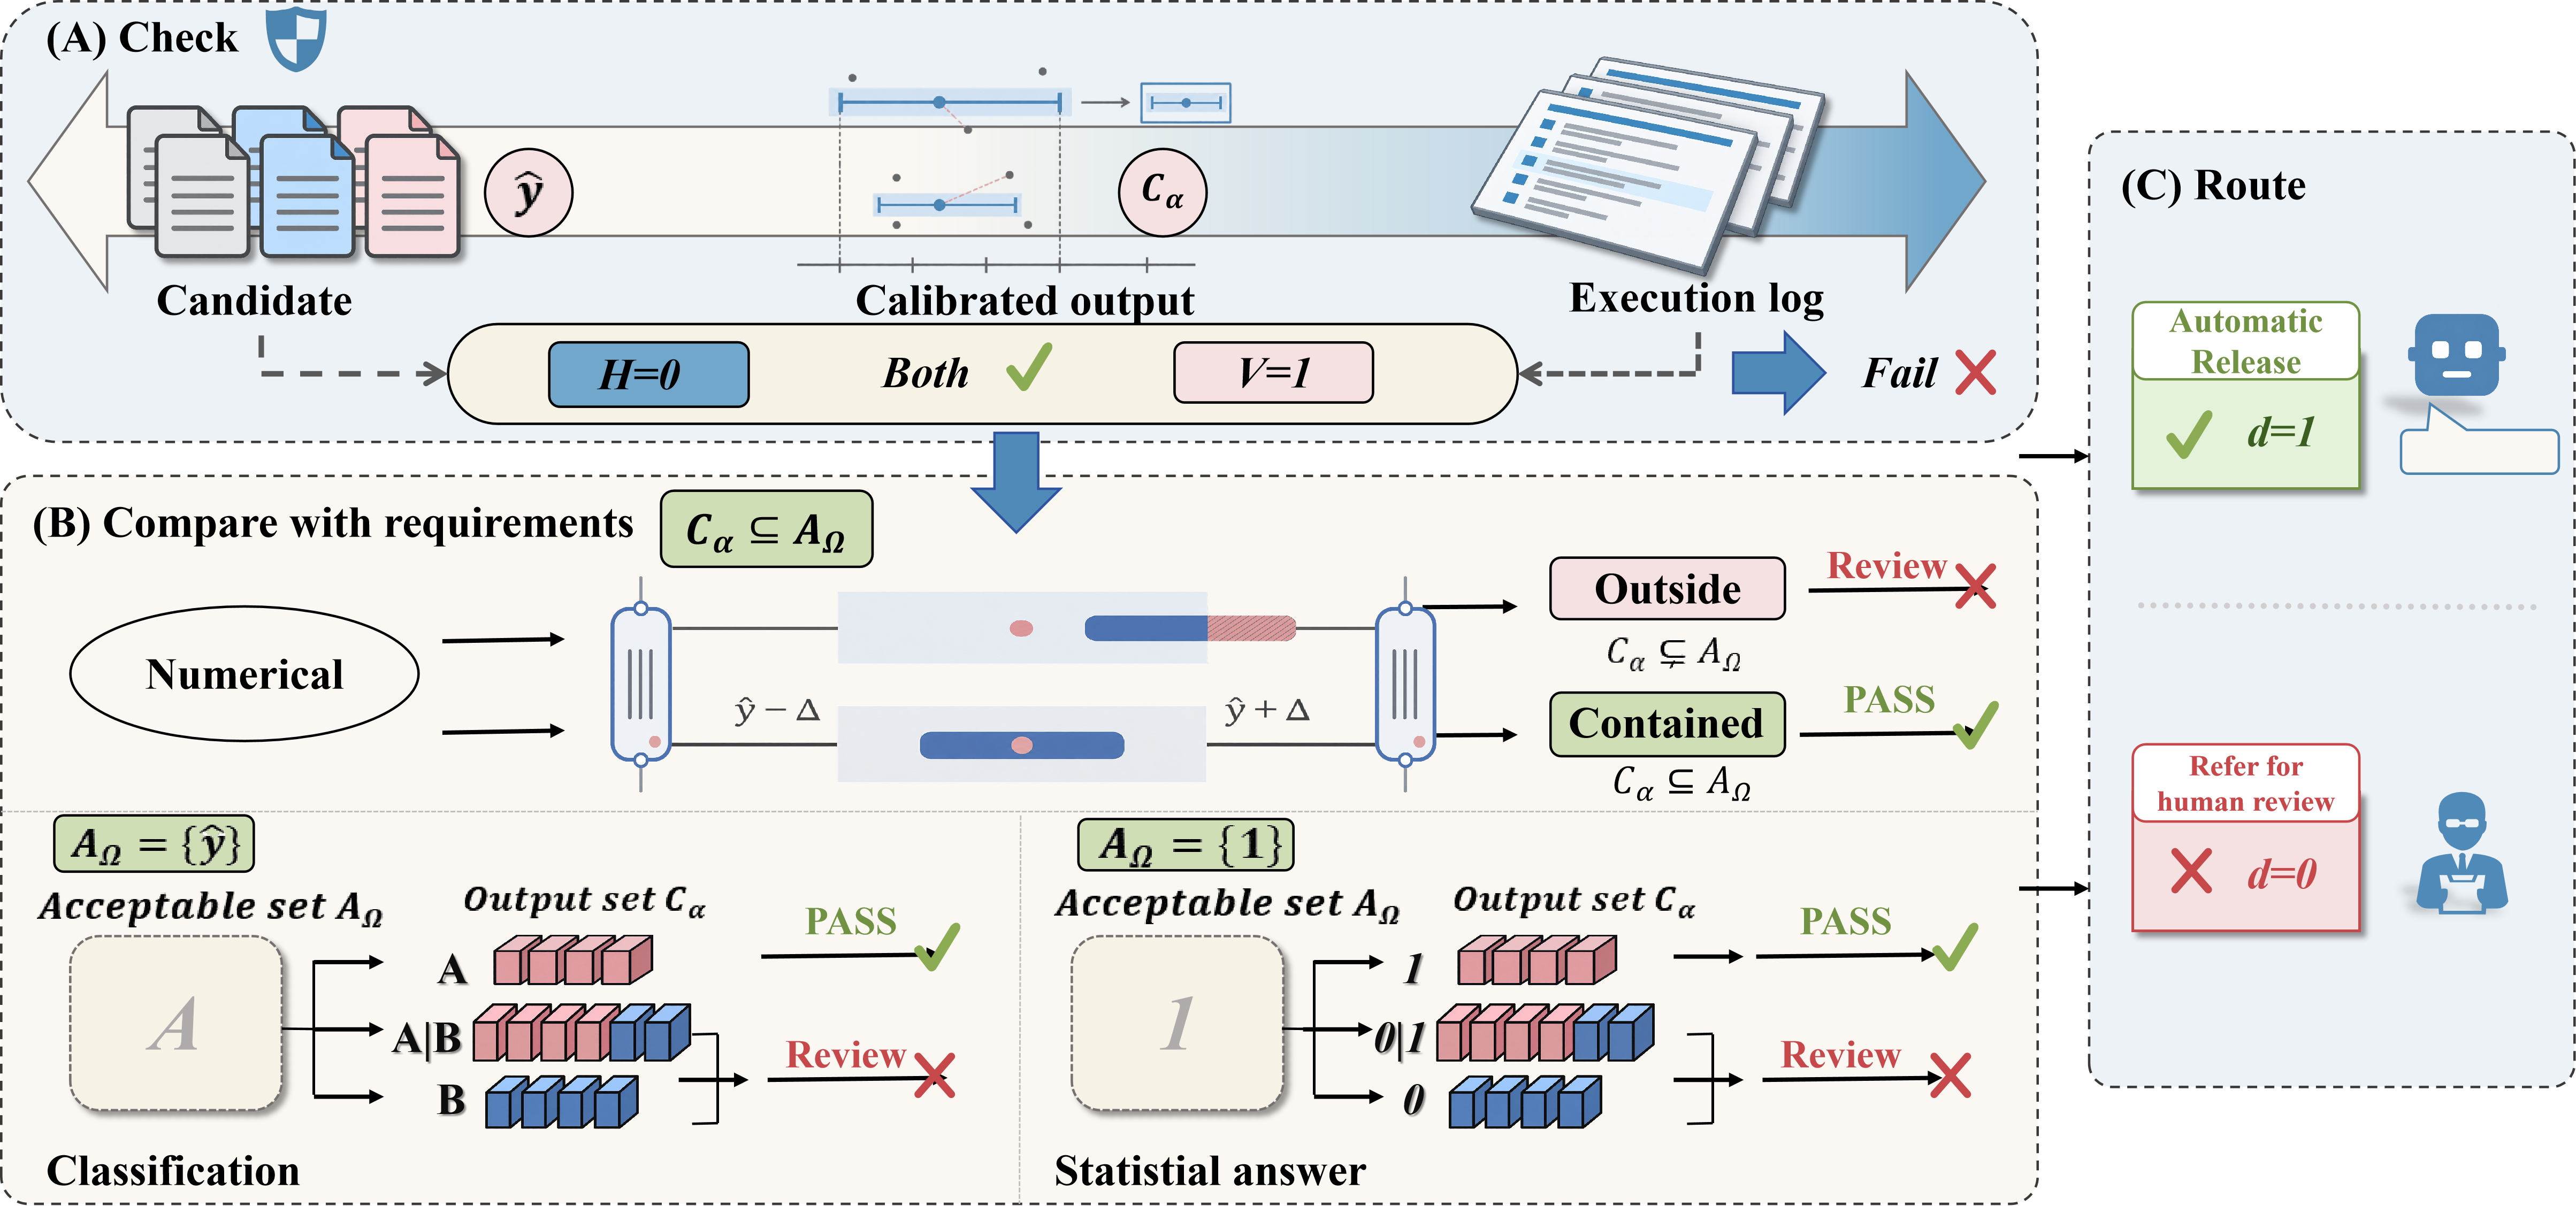
\includegraphics[width=\linewidth]{sci3.png}
    \caption{Risk gating and selective release.}
    \label{fig:risk_gating}
\end{figure}
The containment rule also clarifies the connection between calibration
and release. If \(g_i=1\), then
\(C_i\subseteq\mathcal{A}_{\Omega,i}\); therefore,
\begin{equation}
    \left\{
        g_i=1,\;
        T_i\notin\mathcal{A}_{\Omega,i}
    \right\}
    \subseteq
    \left\{
        T_i\notin C_i
    \right\}.
    \label{eq:release_violation_inclusion}
\end{equation}
Thus, whenever a released result violates the acceptance
criterion, the true target lies outside the calibrated set.
A valid upper bound on marginal miscoverage therefore also
bounds the probability of a release error. The error rate
among released results requires separate evaluation because
it is calculated within the subset selected by the gate
\citep{jin2025confidence}. We therefore report empirical
coverage, release rate, and error rate among released
candidates together.


\section{Experimental Setup}
\label{sec:experimental_setup}

\subsection{Benchmark tasks and datasets}
\label{sec:benchmark_tasks}

Four benchmarks are selected to examine different forms of statistical output and calibrated uncertainty. \textcolor{blue}{StatQA~\citep{zhu2024large} evaluates structured statistical analysis, California Housing~\citep{pace1997sparse} supports numerical regression, Adult~\citep{becker1996adult} supports categorical prediction, and Carbon Monitor~\citep{liu2020carbon} supports temporal forecasting.} Their roles in the evaluation are summarized in Table~\ref{tab:benchmark_tasks}.

\begin{table}[H]
    \centering
    \caption{Benchmark tasks and uncertainty representations}
    \label{tab:benchmark_tasks}
    \small
    \renewcommand{\arraystretch}{1.2}

    \begin{tabularx}{\linewidth}{
        @{}
        >{\raggedright\arraybackslash}p{0.17\linewidth}
        >{\raggedright\arraybackslash}p{0.20\linewidth}
        >{\raggedright\arraybackslash}X
        >{\raggedright\arraybackslash}X
        @{}
    }
        \toprule
        \textbf{Benchmark}
        & \textbf{Task}
        & \textbf{Candidate output}
        & \textbf{Calibrated output} \\
        \midrule

        StatQA
        & Structured statistical analysis
        & Selected variables and statistical methods
        & Correctness-label set \\

        California Housing
        & Numerical regression
        & Point prediction and preliminary quantile interval
        & Conformalized prediction interval \\

        Adult
        & Income classification
        & Predicted class and class probabilities
        & Class prediction set \\

        Carbon Monitor
        & Temporal forecasting
        & Forecast at a fixed horizon
        & Rolling residual-based interval \\

        \bottomrule
    \end{tabularx}
\end{table}

\begin{enumerate}
    \renewcommand{\labelenumi}{\arabic{enumi}.}
    \setlength{\itemsep}{6pt}

    \item \textbf{StatQA.}
    \textcolor{blue}{StatQA~\citep{zhu2024large} is a benchmark for statistical analysis that evaluates the selection of relevant variables and applicable statistical methods. Following the evaluation protocol adopted by the benchmark authors, all experiments on this task are conducted on mini-StatQA, the stratified subset of 1{,}163 examples released together with the benchmark, which preserves the task-category and difficulty distribution of the full collection~\citep{zhu2024large}.} In our evaluation, the candidate answer consists of the variable and method selections returned by the agent. Correctness is determined using the benchmark's official evaluation procedure. This binary outcome also defines the target label for answer-correctness calibration.

    \item \textbf{California Housing.}
    \textcolor{blue}{California Housing~\citep{pace1997sparse}} is used to evaluate numerical prediction of median house values. The statistical tool generates point predictions and preliminary lower and upper quantile estimates, which are subsequently calibrated using conformalized quantile regression. Prediction errors, interval widths, and the allowable error tolerance are reported in consistent target units.

    \item \textbf{Adult.}
    \textcolor{blue}{Adult~\citep{becker1996adult}} is used for binary classification of whether annual income exceeds USD 50,000. The classifier returns a predicted class and class probabilities. These probabilities are converted into a conformal prediction set, allowing the release gate to distinguish a singleton consistent with the predicted class from ambiguous or incompatible outputs.

    \item \textbf{Carbon Monitor.}
    \textcolor{blue}{Carbon Monitor~\citep{liu2020carbon}} provides daily estimates of carbon dioxide emissions and is used here to construct a temporal forecasting task. Forecasts are evaluated at a fixed horizon, and uncertainty is calibrated using previously observed forecast errors.

\end{enumerate}

\subsection{Evaluation metrics}
\label{sec:evaluation_metrics}

The evaluation separates base task performance, calibration
quality, and release decision performance. Base metrics are
computed before gating. Calibration metrics assess the
uncertainty representation, while release metrics assess the
gate's ability to intercept errors and retain correct candidates.

\subsubsection{Base task performance}
\label{sec:base_task_performance}

StatQA is evaluated using the official answer-correctness criterion, and Adult is evaluated using classification accuracy. For both tasks, the overall correctness measure uses all selected test tasks or instances as its denominator.

California Housing and Carbon Monitor are evaluated using mean absolute error (MAE) over valid predictions with observed targets. Failure rates are reported separately.

Let \(N_{\mathrm{test}}\) denote the number of selected test units for a classification or structured-answer task, and let \(b_i=1\) indicate a correct answer and \(b_i=0\) an incorrect or missing answer. The overall correctness rate is
\begin{equation}
    \mathrm{Correctness}
    =
    \frac{1}{N_{\mathrm{test}}}
    \sum_{i=1}^{N_{\mathrm{test}}} b_i.
    \label{eq:exp_correctness}
\end{equation}

For numerical tasks, let \(I_{\mathrm{pred}}\) contain valid
predictions with observed targets. MAE is defined as
\begin{equation}
    \mathrm{MAE}
    =
    \frac{1}{|I_{\mathrm{pred}}|}
    \sum_{i\in I_{\mathrm{pred}}}
    \left|y_i-\hat{y}_i\right|.
    \label{eq:exp_mae}
\end{equation}

\subsubsection{Calibration quality}
\label{sec:exp_calibration_quality}

Calibration is evaluated before release decisions using empirical coverage and output size. Let \(I_{\mathrm{cov}}\) contain results with observed targets and interpretable calibrated outputs. Empirical coverage measures how often the target belongs to its corresponding prediction interval or set:
\begin{equation}
    \widehat{\mathrm{Coverage}}
    =
    \frac{1}{|I_{\mathrm{cov}}|}
    \sum_{i\in I_{\mathrm{cov}}}
    \mathbf{1}\{T_i\in C_i\}.
    \label{eq:exp_coverage}
\end{equation}

Coverage is interpreted relative to the target level \(1-\alpha\), together with mean finite interval width for numerical outputs and mean set cardinality for discrete outputs.

Legitimate empty sets count as noncoverage and are included in set-size statistics. Infinite intervals may be included in coverage diagnostics but are excluded from mean finite width. Calibration failures, empty sets, infinite intervals, and the sizes of the evaluation sets are reported separately.

\subsubsection{Release decision performance}
\label{sec:exp_release_performance}

Release decisions are evaluated against violations of the task-specific acceptance requirements. For numerical tasks, an error means that the absolute prediction error exceeds the prespecified tolerance \(\Delta\). For Adult, an error is an incorrect predicted class. For StatQA, an error is a candidate that fails the official correctness criterion.

Actual error is treated as the positive class, and referral for review as a positive prediction. The resulting confusion matrix is shown in Table~\ref{tab:exp_release_confusion}.

\begin{table}[H]
    \centering
    \caption{Confusion matrix for release decisions}
    \label{tab:exp_release_confusion}
    \footnotesize
    \renewcommand{\arraystretch}{1.2}

    \begin{tabularx}{\linewidth}{
        @{}
        >{\raggedright\arraybackslash}p{0.26\linewidth}
        >{\raggedright\arraybackslash}X
        >{\raggedright\arraybackslash}X
        @{}
    }
        \toprule
        \textbf{System decision}
        & \textbf{Actual error}
        & \textbf{Actual correct} \\
        \midrule

        Referred for review
        & TP: error intercepted
        & FP: correct result withheld \\

        Automatically released
        & FN: error released
        & TN: correct result retained \\

        \bottomrule
    \end{tabularx}
\end{table}

This convention distinguishes successful interception of erroneous outputs from unnecessary withholding of correct outputs.

The primary release metrics are error detection recall, specificity, and balanced accuracy (BA). Recall measures the proportion of erroneous candidates intercepted:
\begin{equation}
    \mathrm{Recall}
    =
    \frac{\mathrm{TP}}
         {\mathrm{TP}+\mathrm{FN}}.
    \label{eq:exp_recall}
\end{equation}

Specificity measures the proportion of correct candidates retained for automatic release:
\begin{equation}
    \mathrm{Specificity}
    =
    \frac{\mathrm{TN}}
         {\mathrm{TN}+\mathrm{FP}}.
    \label{eq:exp_specificity}
\end{equation}

BA assigns equal weight to these objectives:
\begin{equation}
    \mathrm{BA}
    =
    \frac{\mathrm{Recall}+\mathrm{Specificity}}{2}.
    \label{eq:exp_balanced_accuracy}
\end{equation}

We additionally report the automatic release rate and the error rate among released results. The former measures the proportion of evaluable candidates released automatically:
\begin{equation}
    \text{Release rate}
    =
    \frac{\mathrm{TN}+\mathrm{FN}}{N}.
    \label{eq:exp_release_rate}
\end{equation}

The latter measures the proportion of released candidates
that violate the task requirements:
\begin{equation}
    \text{Released error rate}
    =
    \frac{\mathrm{FN}}
         {\mathrm{TN}+\mathrm{FN}}.
    \label{eq:exp_released_error_rate}
\end{equation}

Here, \(N=\mathrm{TP}+\mathrm{FN}+\mathrm{TN}+\mathrm{FP}\) counts common evaluable candidates. Failures without usable candidates and results with missing error labels are reported separately. A release rate over all attempted results is also reported using the total number of registered result units as its denominator.

When both correct and erroneous candidates are present, releasing every candidate or referring every candidate yields a BA of \(0.5\). BA is therefore interpreted jointly with release rate and released error rate. If no candidates are released, the released error rate is reported as N/A. If either actual class is absent, the corresponding recall or specificity and BA are reported as N/A rather than assigned an arbitrary value.

\subsection{Comparative methods}
\label{sec:comparative_methods}

The comparative evaluation includes a reasoning-only baseline, a tool-using baseline, and a conventional release-control baseline. This design separates the benefit of tool-assisted statistical execution from the benefit of calibrated release decisions. The methods and their comparison purposes are summarized in Table~\ref{tab:comparative_methods}.

\begin{table}[H]
    \centering
    \caption{Comparative methods}
    \label{tab:comparative_methods}
    \small
    \renewcommand{\arraystretch}{1.2}

    \begin{tabularx}{\linewidth}{
        @{}
        >{\raggedright\arraybackslash}p{0.24\linewidth}
        >{\raggedright\arraybackslash}X
        >{\raggedright\arraybackslash}p{0.28\linewidth}
        @{}
    }
        \toprule
        \textbf{Method}
        & \textbf{Configuration}
        & \textbf{Comparison purpose} \\
        \midrule

        Zero-shot-CoT
        & Reasoning without statistical tool calls
        & Evaluate tool-assisted execution on StatQA \\

        ReAct Statistical Agent
        & ReAct-style tool use without conformal calibration
          or a release gate
        & Compare base task performance \\

        ReAct with Conventional Gating
        & Tool use with a gate based on uncalibrated intervals
          or confidence scores
        & Compare conventional and conformal release control \\

        TrustStatAgent
        & Explicit planning, statistical tools, conformal
          calibration, and risk gating
        & Evaluate the complete framework \\

        \bottomrule
    \end{tabularx}
\end{table}

\subsection{Ablation studies}
\label{sec:ablation_studies}

Three ablations examine the contributions of explicit planning, conformal calibration, and the risk gate. Each variant removes one component while retaining the other relevant settings.

\textbf{Without explicit planning.}
The agent omits the explicit structured plan but retains the
same task inputs, LLM, statistical tools, and execution budget. This variant is evaluated on StatQA using the official correctness criterion to examine whether explicit planning improves variable and method selection.

\textbf{Without conformal calibration.}
The release procedure uses preliminary intervals or uncalibrated scores instead of conformal outputs. Other prespecified acceptance requirements are retained, and thresholds are not retuned to compensate for removing calibration. This differs from the conventional-gating baseline, which allows threshold selection on validation records. The comparison examines the contribution of calibration under otherwise fixed release settings.

\textbf{Without the risk gate.}
Candidate generation and conformal calibration are retained, but every usable candidate is released automatically. Failures that produce no usable candidate remain execution failures. This variant examines whether the risk gate reduces erroneous releases and how this reduction affects the retention of correct candidates.

The ablation variants and their evaluation focus are summarized in Table~\ref{tab:ablation_design}.

\begin{table}[H]
    \centering
    \caption{Ablation design}
    \label{tab:ablation_design}
    \small
    \renewcommand{\arraystretch}{1.2}

    \begin{tabularx}{\linewidth}{
        @{}
        >{\raggedright\arraybackslash}p{0.27\linewidth}
        >{\raggedright\arraybackslash}p{0.25\linewidth}
        >{\raggedright\arraybackslash}X
        @{}
    }
        \toprule
        \textbf{Variant}
        & \textbf{Removed component}
        & \textbf{Evaluation focus} \\
        \midrule

        w/o Explicit Planning
        & Structured planning
        & StatQA correctness rate \\

        w/o Conformal Calibration
        & Conformal adjustment
        & Recall, specificity, BA, and release statistics \\

        w/o Risk Gate
        & Release filtering
        & Erroneous release and correct-result retention \\

        Full Model
        & None
        & Reference configuration \\

        \bottomrule
    \end{tabularx}
\end{table}
\section{Results and discussion}
\label{sec:results}

\subsection{Experimental settings and reporting protocol}
\label{sec:results_protocol}

This section reports the four benchmarks in three groups.
Section~\ref{sec:results_base} reports base task performance, computed before any release decision is taken.
Section~\ref{sec:results_calibration} reports the quality of the calibrated outputs.
Sections~\ref{sec:results_release} and~\ref{sec:results_ablation} report the release decisions and the ablations.
Tables~\ref{tab:base_performance}--\ref{tab:ablation_results} follow this order, and Figures~\ref{fig:conformal_calibration} and~\ref{fig:risk_gating} fix the procedures whose behaviour these tables measure.
Figures~\ref{fig:candidate_routing}, \ref{fig:cost_ratio} and~\ref{fig:frontier} present the same release decisions in the three forms the discussion relies on, namely their composition, their cost, and their frontier.
The first two are computed from Tables~\ref{tab:release_behaviour} and~\ref{tab:ablation_results} and introduce no additional measurement; the third requires a sweep of the tolerance parameter and is described where it is used.

Release statistics follow the confusion matrix of Table~\ref{tab:exp_release_confusion}, in which an actual violation is the positive class and referral for review is the positive decision, and are computed with Eqs.~\eqref{eq:exp_release_rate} and~\eqref{eq:exp_released_error_rate}.
Each row of Tables~\ref{tab:release_behaviour} and~\ref{tab:ablation_results} is evaluated against the candidate population of the pipeline that produced it, so the released error rate of a row is computed from its own denominator.
Three recorded quantities determine the release statistics reported below: the release rate $r$, the released error rate $e$, and the candidate error rate $p$ of the pipeline that produced the candidates.
The four cells of the confusion matrix follow from them as
$\mathrm{FN}=r\,e$, $\mathrm{TN}=r-\mathrm{FN}$, $\mathrm{TP}=p-\mathrm{FN}$ and $\mathrm{FP}=(1-p)-\mathrm{TN}$,
each expressed as a fraction of the candidate population.
Recall, specificity and balanced accuracy in Eqs.~\eqref{eq:exp_recall}--\eqref{eq:exp_balanced_accuracy} are functions of these four cells, as are the relative reductions of Section~\ref{sec:results_release} and the cost thresholds of Section~\ref{sec:results_discussion}.
The experiment log records $r$ and $e$ for every policy and $p$ for every pipeline, but exports no confusion matrix; the cells above are therefore recovered from the recorded rates rather than tabulated directly, and they are exact consequences of those rates and of the definitions of Eqs.~\eqref{eq:exp_release_rate} and~\eqref{eq:exp_released_error_rate}.
Empirical coverage in Section~\ref{sec:results_calibration} is a separate measurement and is not derived from these three quantities.
Apart from that column, every entry in Tables~\ref{tab:base_performance}--\ref{tab:ablation_results} and in Figures~\ref{fig:candidate_routing} and~\ref{fig:cost_ratio} is either a recorded value of this kind or a quantity derived from one by the relations just stated.
Base metrics cover all selected test units, so a high accuracy cannot arise from withholding difficult cases.
A referred candidate stays in the denominator of the release statistics, which allows a withheld correct result to appear as lower specificity rather than disappearing from the population.
Candidates that yield no usable output are excluded from the release statistics and counted separately as execution failures.
An empty calibrated set is excluded by the validity condition of Eq.~\eqref{eq:unified_release_gate} and counts as noncoverage in Section~\ref{sec:results_calibration}.

The containment rule of Eq.~\eqref{eq:release_violation_inclusion} bounds the joint probability of releasing a violating result.
It does not bound the error rate among released results, which is computed within the subset selected by the gate and requires separate evaluation \citep{jin2025confidence}.
Empirical coverage, release rate, and released error rate are therefore reported together throughout, and no single one of them is used to rank methods.
All operating points, tolerance bands, and acceptance requirements were fixed before the test partition was evaluated; thresholds for conventional gating were selected on the validation split and conformal quantities were computed on the calibration split, as specified in Section~\ref{sec:experimental_setup}.

The four benchmarks are reported separately and are not averaged.
Mean absolute error is expressed in the target unit of its dataset while accuracy is a proportion, and the tasks differ in label noise, set ambiguity, and residual dynamics, so a cross-dataset mean would be governed by scale rather than by behaviour.
Within a benchmark the tables are read in sequence.
Table~\ref{tab:base_performance} describes the candidate population, Table~\ref{tab:calibration_discrimination} the quality of the calibrated output, Table~\ref{tab:release_behaviour} the release decision, and Table~\ref{tab:ablation_results} the contribution of each component.

\subsection{Base task performance}
\label{sec:results_base}

Table~\ref{tab:base_performance} reports the base metrics.
Because the three modules operate after a candidate has been produced, these metrics do not depend on the release decision, and the table compares task competence rather than release behaviour.

TrustStatAgent attains an official accuracy of 72.84\% on StatQA, an accuracy of 84.67\% on Adult, a mean absolute error of 0.3143 on California Housing, and 306.10 on Carbon Monitor.
The first of these is 7.33 percentage points above the same pipeline without explicit planning (Table~\ref{tab:ablation_results}), and it is above the 64.83\% reported by \citet{zhu2024large} for the strongest model \textcolor{blue}{evaluated on the same mini-StatQA subset}.
The latter comparison is not strict.
The present setting supplies a data schema and restricts the analysis to a small fixed set of statistical tools, as illustrated by the workflow of Figure~\ref{fig:planning_execution}, which removes part of the method-selection burden that the benchmark identifies as the dominant error source.
It supports the claim that a tool-restricted agent operates in the regime the benchmark targets; it does not show that the agent surpasses unaided reasoning on the benchmark as originally posed.

The three predictive benchmarks share one statistical tool adapter and one fixed model configuration across methods (Section~\ref{sec:execution}).
On Adult and Carbon Monitor the ReAct and TrustStatAgent pipelines therefore produce identical candidates, at 15.33\% and 3.47\% error, and differ only in the release rule.
On StatQA, where planning changes the analysis itself, the ReAct pipeline releases every candidate at a recorded error rate of 28.23\%, which corresponds to 71.77\% correctness against 72.84\% for the full pipeline.
That difference is worth recording because it is the largest benchmark on which the two pipelines differ in what they compute rather than in what they publish.
California Housing sits between the two cases: the pipelines differ by 0.12 percentage points, 4.51\% against 4.38\%, which is small relative to StatQA and is treated below as a difference in the candidate population rather than as a property of the gate.

The same table fixes the population on which the gate has to work.
The candidate error rate of the full pipeline is 27.16\% on StatQA, 15.33\% on Adult, 4.38\% on California Housing, and 3.47\% on Carbon Monitor, a range of almost one order of magnitude.
The publish-every-candidate baseline of Table~\ref{tab:release_behaviour} is the ReAct pipeline, whose candidate error rate is 28.23\% on StatQA and 4.51\% on California Housing; the variant without the gate in Table~\ref{tab:ablation_results} uses the full pipeline and yields 27.16\% and 4.38\%.
The two rows differ in the pipeline that generated the candidates, not in the release rule.
Most of the variation reported in Sections~\ref{sec:results_release} and~\ref{sec:results_discussion} follows from this range rather than from the gate, and the four tasks are best read as four different operating regimes.

\begin{table}[t]
\centering
\small
\caption{Base task performance before any release decision. Metrics are computed over all selected test units and are therefore unaffected by referral. MAE is reported in the unit of the corresponding dataset, as defined by that benchmark. The ReAct accuracy on StatQA is the complement of its recorded released error rate, 28.23\%, because that entry releases every candidate. Entries marked $\dagger$ coincide with the TrustStatAgent value because the three predictive benchmarks use the same tool adapter and model configuration in every variant (Section~\ref{sec:execution}).}
\label{tab:base_performance}
\begin{tabularx}{\linewidth}{@{}lccc@{}}
\toprule
\textbf{Benchmark} & \textbf{Base metric} & \textbf{ReAct agent} & \textbf{TrustStatAgent}\\
\midrule
StatQA & Official accuracy (\%) & 71.77 & 72.84\\
Adult & Accuracy (\%) & 84.67$^\dagger$ & 84.67\\
California Housing & MAE & 0.3143$^\dagger$ & 0.3143\\
Carbon Monitor & MAE & 306.10$^\dagger$ & 306.10\\
\bottomrule
\end{tabularx}
\end{table}

\subsection{Quality of the calibrated outputs}
\label{sec:results_calibration}

Figure~\ref{fig:conformal_calibration} summarises the four constructions whose outputs are evaluated here: conformalized quantile regression for California Housing, probability-threshold sets for Adult, the correctness-set construction for StatQA, and the rolling residual interval for Carbon Monitor.

Empirical coverage is 98.53\% on Adult, 84.23\% on California Housing and 92.08\% on Carbon Monitor.
Coverage on StatQA is not reported here because the export on which this section is based does not include it.
Two features of the construction make the realised value conservative with respect to the level the procedure targets.
The rank $k_\alpha$ in Eq.~\eqref{eq:calibration_threshold} is rounded up and truncated at $n$, so the largest observed score replaces an order statistic that may be unattainable, and both adjustments are conservative for a finite calibration sample.
For California Housing the correction in Eq.~\eqref{eq:cqr_calibrated_interval} is additionally nonnegative, so calibration can widen the preliminary interval but never narrow it.
The nominal level is selected per task on the validation split, and the realised coverage is reported as a diagnostic of the calibrated output.
Under-coverage would be the more damaging outcome whatever that level is, because the release conditions of Table~\ref{tab:calibrated_release_conditions} are stated in terms of the calibrated output.

Coverage on Carbon Monitor should be read as a diagnostic rather than as an instance of the guarantee.
The rolling rule of Eqs.~\eqref{eq:rolling_residual_scores}--\eqref{eq:rolling_calibrated_interval} conditions on the recent residual scale, so the exchangeability assumption behind the marginal guarantee is not asserted for this task; online conformal methods treat this setting explicitly \citep{angelopoulos2024online}.
The realised 92.08\% describes behaviour under the drift present in the evaluation period.

Coverage and released correctness diverge, and they diverge in opposite directions on the two task families.
On California Housing coverage is 84.23\% while released correctness is 98.13\%.
Release there requires both endpoints of the calibrated interval to lie inside the tolerance band of Eq.~\eqref{eq:numerical_acceptance_set}, so only candidates with a narrow interval, and therefore a small error, reach publication.
On Adult the order reverses, with coverage at 98.53\% and released correctness at 97.28\%.
Release there requires the calibrated set to equal the predicted-class singleton, Eq.~\eqref{eq:categorical_prediction_set}, which measures ambiguity rather than error magnitude, and a confident singleton is not necessarily a correct one.
The distinction between the width-based condition of Figure~\ref{fig:conformal_calibration}A and the singleton-based condition of Figure~\ref{fig:conformal_calibration}B accounts for most of the differences in gate performance reported below.

\begin{table}[t]
\centering
\scriptsize
\caption{Calibration quality and discrimination of the release decision for TrustStatAgent. Coverage, Eq.~\eqref{eq:exp_coverage}, is computed over all candidates with interpretable calibrated outputs, whereas recall, specificity, and balanced accuracy, Eqs.~\eqref{eq:exp_recall}--\eqref{eq:exp_balanced_accuracy}, are computed over the confusion matrix of Table~\ref{tab:exp_release_confusion}. Every row uses the candidate population of the pipeline that produced it, namely the without-gate row of Table~\ref{tab:ablation_results}: 27.16\% on StatQA, 15.33\% on Adult, 4.38\% on California Housing and 3.47\% on Carbon Monitor. Using the ReAct population instead would change the StatQA and California Housing rows only, by at most one percentage point. The nominal level is selected per task on the validation split. Coverage on StatQA is not available in the exported results and is marked accordingly. Publishing every candidate attains recall 0, specificity 1, and BA 0.5 on every benchmark. The last column gives the number of correct results withheld per intercepted error.}
\label{tab:calibration_discrimination}
\setlength{\tabcolsep}{3pt}
\begin{tabularx}{\linewidth}{@{}lccccc@{}}
\toprule
\textbf{Benchmark} & \textbf{Coverage (\%)} & \textbf{Recall (\%)} & \textbf{Specificity (\%)} & \textbf{BA} & \textbf{Referrals per error}\\
\midrule
StatQA & --- & 96.83 & 62.13 & 0.795 & 1.05\\
Adult & 98.53 & 90.39 & 62.38 & 0.764 & 2.30\\
Calif. Housing & 84.23 & 72.93 & 65.32 & 0.691 & 10.37\\
Carbon Monitor & 92.08 & 28.57 & 77.95 & 0.533 & 21.50\\
\bottomrule
\end{tabularx}
\end{table}

\subsection{Release decisions}
\label{sec:results_release}

Table~\ref{tab:release_behaviour} reports the release rate and the released error rate of the three policies.
Publishing every candidate reproduces the candidate error rate of the pipeline that produced it and serves as the upper bound on automation.
The two baselines of Tables~\ref{tab:release_behaviour} and~\ref{tab:ablation_results} differ by 1.07 percentage points on StatQA and 0.12 on California Housing because they are the same policy applied to the ReAct and full candidate pools, as Section~\ref{sec:results_base} explains.
Figure~\ref{fig:risk_gating} shows the routing that produces these numbers: a candidate is released only when execution succeeds, the uncertainty output is valid, and the acceptance test of Table~\ref{tab:calibrated_release_conditions} is met, and every referred candidate carries the condition it failed.
Figure~\ref{fig:candidate_routing} decomposes the same decision into the four outcomes of the confusion matrix of Table~\ref{tab:exp_release_confusion}.
Each block describes one candidate population twice: it is first released without the gate and then passed through it.
Because the boundary between error-related and correct-related segments falls at the same position in both bars, the figure shows that the gate reallocates candidates within a fixed error budget instead of altering it.
What differs across benchmarks is where the reallocation lands, and that is the subject of the rest of this section.

TrustStatAgent attains the lowest released error rate on all four benchmarks: 1.87\% on StatQA, 2.72\% on Adult, 1.87\% on California Housing, and 3.18\% on Carbon Monitor, against 1.96\%, 3.22\%, 2.02\%, and 3.93\% for conventional gating.
Relative to publishing every candidate from the same pipeline, this is a reduction of 93.1\%, 82.3\%, 57.5\%, and 8.1\%.
The four cases differ in what that reduction costs, and the difference is informative.

On StatQA the calibration gain comes free.
The gate reduces the released error rate from 27.16\% (the same pipeline publishing everything, Table~\ref{tab:ablation_results}) to 1.87\% while releasing 46.12\% of candidates, 2.16 percentage points more than conventional gating, which releases 43.97\%.
The gap in released error rate to conventional gating is 0.09 percentage points, which is small and is discussed in Section~\ref{sec:results_limitations}; what the two operating points establish is that calibration need not trade automation for reliability on this task.

Adult shows the case in which the gate acts on ambiguity.
It releases 54.29\% of predictions with a released error rate of 2.72\%, whereas conventional gating releases 57.18\% at 3.22\%.
The released subset retains 97.28\% correctness against 84.67\% for the unrestricted baseline, and 90.39\% of the erroneous candidates are intercepted.
The cost appears in the referral load: 45.71\% of the population is referred, of which 31.85\% are correct results withheld for review, or 2.3 unnecessary referrals per intercepted error.
The calibrated rule therefore gives up 2.9 percentage points of automation to remove half a percentage point of error, an exchange worth making only if a referral is much cheaper than a published mistake.

On California Housing the interval width carries information about error magnitude, and the gate uses it directly.
It releases 63.64\% of cases with a released error rate of 1.87\% and intercepts 72.93\% of violating predictions, against 67.22\% released at 2.02\% for conventional gating.
The trade is 3.6 percentage points of automation for 0.15 percentage points of error, and the referral ratio makes the price explicit: 33.16\% of the population are correct results withheld, or 10.4 referrals per intercepted error.
A gate that intercepts most of a small violating subset necessarily withholds a larger absolute number of correct results.

Carbon Monitor separates the policies most sharply, and the comparison is not a trade at all.
Conventional gating releases 88.12\% of forecasts and intercepts none of the 3.47\% violating ones, so its released error rate, 3.93\%, is higher than that of publishing everything; it withholds 11.88\% of the population without removing a single error.
We attribute this to the structure of the task rather than to the threshold value.
The forecaster is the previous observation (Section~\ref{sec:uncertainty_calibration}), so the interval of Eq.~\eqref{eq:rolling_calibrated_interval} reflects nothing but the recent residual scale.
When the series has been calm the interval is narrow, and a level shift then produces a large error together with a narrow interval.
A rule that responds to width therefore misses exactly the errors that follow calm periods, and a threshold tuned on validation records inherits the same failure because it responds to the same quantity.
The calibrated rule intercepts 28.57\% of violations and releases 77.72\% at 3.18\%, which is 10.4 percentage points fewer forecasts than the conventional policy.

Across the four benchmarks the same rule releases between 46.12\% and 77.72\% of candidates.
The spread is intended.
The rule publishes the subset whose calibrated output satisfies the acceptance region of its task and imposes no publication quota, so the released fraction follows the uncertainty of the task.

\begin{table}[t]
\centering
\scriptsize
\caption{Release behaviour of the three policies on the test partition. Publishing every candidate reproduces the candidate error rate of Table~\ref{tab:base_performance}. Conventional gating applies a threshold tuned on validation records to uncalibrated intervals or confidence scores.}
\label{tab:release_behaviour}
\setlength{\tabcolsep}{3pt}
\begin{tabularx}{\linewidth}{@{}lcccccc@{}}
\toprule
& \multicolumn{2}{c}{\textbf{Publish every candidate}} & \multicolumn{2}{c}{\textbf{Conventional gating}} & \multicolumn{2}{c}{\textbf{TrustStatAgent}}\\
\cmidrule(lr){2-3}\cmidrule(lr){4-5}\cmidrule(lr){6-7}
\textbf{Benchmark} & Release (\%) & Error (\%) & Release (\%) & Error (\%) & Release (\%) & Error (\%)\\
\midrule
StatQA & 100.00 & 28.23 & 43.97 & 1.96 & 46.12 & 1.87\\
Adult & 100.00 & 15.33 & 57.18 & 3.22 & 54.29 & 2.72\\
Calif. Housing & 100.00 & 4.51 & 67.22 & 2.02 & 63.64 & 1.87\\
Carbon Monitor & 100.00 & 3.47 & 88.12 & 3.93 & 77.72 & 3.18\\
\bottomrule
\end{tabularx}
\end{table}

\begin{figure}[t]
\centering
\providecolor{cHit}{RGB}{24,95,165}%
\providecolor{cErr}{RGB}{163,45,45}%
\providecolor{cOk}{RGB}{192,221,151}%
\providecolor{cHold}{RGB}{186,117,23}%
\begin{tikzpicture}[x=0.085cm,y=1cm]

\fill[cErr] (0,0) rectangle (27.155,0.30);
\fill[cOk] (27.155,0) rectangle (100,0.30);
\node[font=\footnotesize,text=white] at (13.58,0.15) {27.2};
\node[font=\footnotesize] at (63.58,0.15) {72.8};
\node[anchor=west,font=\footnotesize,text=black!55] at (101.8,0.15) {w/o gate};

\fill[cHit] (0,-0.42) rectangle (26.293,-0.12);
\fill[cErr] (26.293,-0.42) rectangle (27.155,-0.12);
\fill[cOk] (27.155,-0.42) rectangle (72.414,-0.12);
\fill[cHold] (72.414,-0.42) rectangle (100,-0.12);
\node[font=\footnotesize,text=white] at (13.15,-0.27) {26.3};
\node[font=\footnotesize] at (49.78,-0.27) {45.3};
\node[font=\footnotesize,text=white] at (86.21,-0.27) {27.6};
\node[anchor=west,font=\footnotesize,text=black!55] at (101.8,-0.27) {gated};

\node[anchor=east,font=\footnotesize] at (-2,-0.06) {StatQA};

\draw[black!12,line width=0.4pt] (0,-0.835) -- (100,-0.835);

\fill[cErr] (0,-1.55) rectangle (15.332,-1.25);
\fill[cOk] (15.332,-1.55) rectangle (100,-1.25);
\node[font=\footnotesize,text=white] at (7.67,-1.40) {15.3};
\node[font=\footnotesize] at (57.67,-1.40) {84.7};

\fill[cHit] (0,-1.97) rectangle (13.858,-1.67);
\fill[cErr] (13.858,-1.97) rectangle (15.332,-1.67);
\fill[cOk] (15.332,-1.97) rectangle (68.147,-1.67);
\fill[cHold] (68.147,-1.97) rectangle (100,-1.67);
\node[font=\footnotesize,text=white] at (6.93,-1.82) {13.9};
\node[font=\footnotesize] at (41.74,-1.82) {52.8};
\node[font=\footnotesize,text=white] at (84.07,-1.82) {31.9};

\node[anchor=east,font=\footnotesize] at (-2,-1.61) {Adult};

\draw[black!12,line width=0.4pt] (0,-2.385) -- (100,-2.385);

\fill[cErr] (0,-3.10) rectangle (4.385,-2.80);
\fill[cOk] (4.385,-3.10) rectangle (100,-2.80);
\node[font=\footnotesize] at (52.19,-2.95) {95.6};

\fill[cHit] (0,-3.52) rectangle (3.198,-3.22);
\fill[cErr] (3.198,-3.52) rectangle (4.385,-3.22);
\fill[cOk] (4.385,-3.52) rectangle (66.836,-3.22);
\fill[cHold] (66.836,-3.52) rectangle (100,-3.22);
\node[font=\footnotesize] at (35.61,-3.37) {62.5};
\node[font=\footnotesize,text=white] at (83.42,-3.37) {33.2};

\node[anchor=east,font=\footnotesize] at (-2,-3.16) {California Housing};

\draw[black!12,line width=0.4pt] (0,-3.935) -- (100,-3.935);

\fill[cErr] (0,-4.65) rectangle (3.465,-4.35);
\fill[cOk] (3.465,-4.65) rectangle (100,-4.35);
\node[font=\footnotesize] at (51.73,-4.50) {96.5};

\fill[cHit] (0,-5.07) rectangle (0.990,-4.77);
\fill[cErr] (0.990,-5.07) rectangle (3.465,-4.77);
\fill[cOk] (3.465,-5.07) rectangle (78.713,-4.77);
\fill[cHold] (78.713,-5.07) rectangle (100,-4.77);
\node[font=\footnotesize] at (41.09,-4.92) {75.2};
\node[font=\footnotesize,text=white] at (89.36,-4.92) {21.3};

\node[anchor=east,font=\footnotesize] at (-2,-4.71) {Carbon Monitor};

\fill[cHit] (0,-5.97) rectangle (3.1,-5.73);
\node[anchor=west,font=\footnotesize] at (4.0,-5.85) {error intercepted};
\fill[cErr] (46,-5.97) rectangle (49.1,-5.73);
\node[anchor=west,font=\footnotesize] at (50,-5.85) {error released};

\fill[cOk] (0,-6.42) rectangle (3.1,-6.18);
\node[anchor=west,font=\footnotesize] at (4.0,-6.30) {correct released};
\fill[cHold] (46,-6.42) rectangle (49.1,-6.18);
\node[anchor=west,font=\footnotesize] at (50,-6.30) {correct withheld};
\end{tikzpicture}
\caption{Composition of the release decision. Each block describes one candidate population twice: released without the gate in the upper bar, released through the gate in the lower bar. Bar lengths are percentages of the population. The boundary between error-related and correct-related segments falls at the same position in both bars of a block, so the gate reallocates candidates within a fixed error budget rather than changing it; the numbers are those of Table~\ref{tab:ablation_results}, without-gate row, decomposed with Eqs.~\eqref{eq:exp_release_rate} and~\eqref{eq:exp_released_error_rate}. Segments narrower than five percent are left unlabelled; the four populations contain 27.16\%, 15.33\%, 4.38\% and 3.47\% errors, which is the length of the red block in each upper bar. On Carbon Monitor the released error segment (2.48\%) is longer than the intercepted one (0.99\%), and the withheld segment (21.29\%) is the smallest of the four, so the gate is least active on the benchmark where its detection is weakest.}
\label{fig:candidate_routing}
\end{figure}

\subsection{Ablation results}
\label{sec:results_ablation}

Table~\ref{tab:ablation_results} isolates the three components.
Removing explicit planning lowers StatQA accuracy from 72.84\% to 65.52\%, a difference of 7.33 percentage points under the official criterion.
The plan helps because it is an executable intermediate representation rather than a narrative.
It records the task type, the response variable, the selected inputs, the method, the preprocessing, and the tool sequence, and each field is later checked against the execution log.
Without it the agent still calls the tools, but variable and method selection become implicit and are correspondingly harder to verify.

Removing the gate releases every candidate that holds a valid calibrated output.
The released error rate then becomes 27.16\% on StatQA, 15.33\% on Adult, 4.38\% on California Housing, and 3.47\% on Carbon Monitor.
These values reproduce the candidate error rates of Section~\ref{sec:results_base}, as they must when no candidate is withheld; for StatQA and Adult they are also the complements of the accuracies in Table~\ref{tab:base_performance}.
The agreement confirms that the release statistics and the base metrics share a denominator, and that the gate is the only source of selectivity in Table~\ref{tab:release_behaviour}.

Removing calibration raises the released error rate on StatQA from 1.87\% to 5.93\%, a factor of 3.2.
On Adult and Carbon Monitor the variant degenerates to unrestricted publication, at 100\% release and the candidate error rate of 15.33\% and 3.47\%, for a structural reason.
The acceptance conditions of Table~\ref{tab:calibrated_release_conditions} are stated on the calibrated output, so without calibration the preset requirements cannot be evaluated and the gate defaults to release.
The variant was not retuned, as specified in Section~\ref{sec:ablation_studies}, since allowing the threshold to be re-optimised would reintroduce the validation tuning that the comparison is meant to isolate.
California Housing is the informative exception: there the variant still releases 64.39\% of candidates at 1.88\%, marginally more candidates and marginally more errors than the full model, because the preliminary quantile interval already has approximately the scale that the tolerance band requires.
Calibration therefore contributes least where the uncalibrated interval is already close to the acceptance region, which is what the construction of Eq.~\eqref{eq:cqr_calibrated_interval} predicts.

The two reliability modules are complementary rather than substitutable.
Calibration supplies a scale on which a violation can be measured, and the gate turns that scale into a decision.
Calibration alone does not decide publication, since a valid interval can still fall outside the tolerance band; gating without calibration has no quantity to threshold, which is why two of the three predictive benchmarks collapse to release-all.
The behaviour of conventional gating on Carbon Monitor agrees with this reading: it is a gate applied to an uncalibrated scale, and it intercepts nothing when that scale stops tracking the error.

\begin{table}[t]
\centering
\scriptsize
\caption{Ablation results. The variant without the gate releases every candidate that holds a valid calibrated output, so its released error rate reproduces the candidate error rate of Section~\ref{sec:results_base}.}
\label{tab:ablation_results}
\setlength{\tabcolsep}{3pt}
\begin{tabularx}{\linewidth}{@{}llcccc@{}}
\toprule
\textbf{Variant} & \textbf{Metric} & \textbf{StatQA} & \textbf{Adult} & \textbf{Calif. Housing} & \textbf{Carbon Monitor}\\
\midrule
Publish all (ReAct) & Released err. (\%) & 28.23 & 15.33 & 4.51 & 3.47\\
w/o Risk Gate & Released err. (\%) & 27.16 & 15.33 & 4.38 & 3.47\\
w/o Conformal Calib. & Released err. (\%) & 5.93 & 15.33 & 1.88 & 3.47\\
Full Model & Released err. (\%) & 1.87 & 2.72 & 1.87 & 3.18\\
\midrule
w/o Explicit Planning & Accuracy (\%) & 65.52 & --- & --- & ---\\
Full Model & Accuracy (\%) & 72.84 & --- & --- & ---\\
\bottomrule
\end{tabularx}
\end{table}

\subsection{Discussion}
\label{sec:results_discussion}

The four benchmarks divide the work of the gate in a consistent way, and the division follows two properties of the task rather than any implementation detail.

The first is the base error rate.
Balanced accuracy is 0.795 on StatQA at a 27.16\% base rate, 0.764 on Adult at 15.33\%, 0.691 on California Housing at 4.38\%, and 0.533 on Carbon Monitor at 3.47\%.
Intercepting a rare violation without withholding most correct results is a harder discrimination problem than intercepting a frequent one, and the ranking follows the base rate closely.
On Carbon Monitor, 0.533 is barely above the 0.5 attained by publishing everything, so the reliability argument on that task rests on calibrated coverage and on the fact that the conventional rule intercepts nothing, rather than on the discriminative power of the gate.
The second property is the form of the acceptance condition.
A width-based condition is approximately monotone in the error magnitude, which is why California Housing intercepts 72.93\% of violations from a base rate of only 4.38\%, whereas a singleton condition responds to ambiguity and separates confident correct predictions from confident incorrect ones much less sharply.

Balanced accuracy, however, separates the two gates only where the base rate is high or the competing scale is broken: 0.795 against 0.785 on StatQA and 0.533 against 0.438 on Carbon Monitor.
On Adult and California Housing the two rules sit within 0.005 of each other (0.764 against 0.767, and 0.691 against 0.694), so the aggregate discrimination is effectively the same and the difference appears in where the operating point sits: the calibrated rule intercepts slightly more violations and withholds slightly more correct results.
This is why the released error rate and the release rate are reported as a pair rather than through a single discriminative score.

These two properties also define the trade-off that the release decision has to resolve.
Tightening the tolerance parameter $\Delta$ withholds more results and lowers the released error rate, while loosening it does the reverse.
The two quantities therefore cannot be improved together by moving a single threshold, and Fig.~\ref{fig:frontier} traces the frontier obtained when $\Delta$ is swept with the rest of the pipeline fixed.
Read as a frontier, the comparison in Section~\ref{sec:results_release} supports a specific claim.
On StatQA the calibrated rule dominates the conventional one at the reported operating point, releasing more while erring less.
On the other three benchmarks it moves along the frontier rather than pushing it, buying 0.15 to 0.75 percentage points of released error with 2.9 to 10.4 percentage points of automation.
On Carbon Monitor the conventional policy is not on the frontier at all: it releases less than publishing everything and errs more, because it intercepts no violations.
A point of that kind cannot be a conservative choice; it is a threshold applied to the wrong quantity.

The relative weight of the two quantities belongs to the deployment rather than to the method.
Let $c_e$ be the cost of a published violation and $c_r$ the cost of one referral.
The expected cost per candidate is proportional to $c_e\,r\,e + c_r\,(1-r)$, where $r$ is the release rate and $e$ the released error rate.
The ratio at which the reported operating point becomes cheaper than publishing everything follows from the same expression and equals $\rho^{\ast}=(1-r)/(p-r\,e)$, which is 2.05 on StatQA, 3.30 on Adult, 11.0 on California Housing, and 22.5 on Carbon Monitor.
Figure~\ref{fig:cost_ratio} plots the comparison on which these numbers rest.
The relative cost falls monotonically in the ratio, crosses parity at the quoted value, and then flattens at a level fixed by the two error rates, so the threshold is a property of the operating point rather than of the cost model.
These thresholds are modest.
On the two tasks where a violation is common, a published error need only cost two to three times a referral for the gate to pay for itself.
On the two numerical tasks, violations are rare and most referrals are unnecessary, so the same argument requires an order of magnitude more.
The comparison with conventional gating resolves in the same way.
Writing $r_c$ and $e_c$ for its recorded rates, the calibrated rule is cheaper once the ratio exceeds $\rho=(r-r_c)/(r\,e-r_c\,e_c)$; the denominator vanishes on StatQA, where the two error products coincide, so the calibrated rule is cheaper at every ratio there.
On the other three benchmarks the value is 7.9 on Adult, 21.1 on California Housing and 10.5 on Carbon Monitor.
The referral load implied by the reported operating points is 53.88\% of the population on StatQA, 45.71\% on Adult, 36.36\% on California Housing, and 22.28\% on Carbon Monitor, which is the quantity an operator would size review capacity against.

Two implications follow for the design of expert systems.
The first concerns where the release decision is taken.
In this workflow the decision is made by a program whose inputs, namely the execution log, the calibrated output, and the acceptance region, are inspectable and can be attached to the referral; a system that asks the model to report its own confidence has no equivalent audit trail.
The second concerns the isolation of the calibration set.
Because the calibration split is excluded from model fitting and its labels never reach the LLM, the marginal guarantee refers to a procedure rather than to the model's self-assessment, which is what distinguishes a calibrated gate from a threshold applied to a heuristic score.

The results also locate the contribution relative to existing work.
Selective prediction formalises the risk--coverage trade-off used here \citep{geifman2017selective,elyaniv2010foundations}, and selective generation applies it to language models \citep{lee2024selective}.
Conformal language modelling constructs output sets with coverage guarantees \citep{quach2024conformal,wang2024conu,cherian2024large}, and recent work examines how such sets can be made informative \citep{gazin2025selecting} and how coverage behaves after selection \citep{jin2025confidence}.
The difference is in what the calibrated quantity is attached to.
In those settings the conformal set describes the uncertainty of a generated answer; here it describes the uncertainty of a computational result whose execution can also be checked, and the release rule of Eq.~\eqref{eq:unified_release_gate} requires both.
That combination has a practical consequence.
The failure of conventional gating on Carbon Monitor is not a failure of threshold tuning but of applying a width signal to a quantity that no longer tracks the error, which is the condition that an execution-grounded calibration can register.

\begin{figure}[t]
\centering
\providecolor{cS}{RGB}{24,95,165}%
\providecolor{cA}{RGB}{15,110,86}%
\providecolor{cH}{RGB}{186,117,23}%
\providecolor{cC}{RGB}{83,74,183}%
\begin{tikzpicture}[x=4.0cm,y=0.55cm]

\draw[black!45,line width=0.4pt] (0,0) -- (2.06,0);
\draw[black!45,line width=0.4pt] (0,0) -- (0,9.35);

\foreach \v/\l in {0/1,0.301/2,0.699/5,1/10,1.301/20,1.699/50,2/100}{
  \draw[black!45,line width=0.4pt] (\v,0) -- (\v,-0.16) node[below,font=\scriptsize,inner sep=1pt] {\l};
}
\foreach \v in {2,4,6,8}{
  \draw[black!45,line width=0.4pt] (0,\v) -- (-0.018,\v) node[left,font=\scriptsize,inner sep=1pt] {\v};
}

\node[below,font=\footnotesize] at (1.0,-1.55) {cost of a published violation $\div$ cost of a referral};
\node[rotate=90,font=\footnotesize] at (-0.24,4.7) {expected cost, gate $\div$ publish all};

\draw[black!55,dashed,line width=0.5pt] (0,1) -- (2.04,1);
\node[above,font=\scriptsize,text=black!60] at (1.74,1.06) {break-even};

\draw[cS,line width=0.9pt,mark=none] plot coordinates {(0,2.016) (0.079,1.685) (0.176,1.354) (0.301,1.024) (0.398,0.825) (0.477,0.693) (0.602,0.528) (0.699,0.429) (0.778,0.362) (0.903,0.280) (1,0.230) (1.176,0.164) (1.301,0.131) (1.477,0.098) (1.699,0.071) (1.845,0.060) (2,0.052)};
\draw[cA,line width=0.9pt,mark=none] plot coordinates {(0,3.077) (0.079,2.581) (0.176,2.084) (0.301,1.587) (0.398,1.289) (0.477,1.090) (0.519,1.000) (0.602,0.842) (0.699,0.692) (0.778,0.593) (0.903,0.469) (1,0.394) (1.176,0.295) (1.301,0.245) (1.477,0.196) (1.699,0.156) (1.845,0.139) (2,0.126)};
\draw[cH,line width=0.9pt,mark=none] plot coordinates {(0,8.333) (0.079,6.988) (0.176,5.643) (0.301,4.298) (0.398,3.491) (0.477,2.953) (0.602,2.281) (0.699,1.877) (0.778,1.608) (0.903,1.272) (1,1.070) (1.041,0.997) (1.176,0.802) (1.301,0.667) (1.477,0.532) (1.699,0.425) (1.845,0.379) (2,0.344)};
\draw[cC,line width=0.9pt,mark=none] plot coordinates {(0,7.143) (0.079,6.072) (0.176,5.000) (0.301,3.929) (0.477,2.857) (0.602,2.321) (0.699,2.000) (0.778,1.786) (0.903,1.518) (1,1.357) (1.176,1.143) (1.301,1.036) (1.352,1.000) (1.477,0.929) (1.602,0.875) (1.699,0.843) (1.845,0.806) (2,0.779)};

\fill[white] (0.312,1) circle (2.2pt);
\draw[cS,line width=0.9pt] (0.312,1) circle (2.2pt);
\fill[white] (0.519,1) circle (2.2pt);
\draw[cA,line width=0.9pt] (0.519,1) circle (2.2pt);
\fill[white] (1.041,1) circle (2.2pt);
\draw[cH,line width=0.9pt] (1.041,1) circle (2.2pt);
\fill[white] (1.352,1) circle (2.2pt);
\draw[cC,line width=0.9pt] (1.352,1) circle (2.2pt);

\node[below,font=\scriptsize,text=cS] at (0.312,0.74) {2.05};
\node[below,font=\scriptsize,text=cA] at (0.519,0.74) {3.30};
\node[below,font=\scriptsize,text=cH] at (1.041,0.74) {11.0};
\node[below,font=\scriptsize,text=cC] at (1.352,0.74) {22.5};

\draw[cS,line width=0.9pt] (1.28,8.60) -- (1.38,8.60);
\node[anchor=west,font=\scriptsize] at (1.41,8.60) {StatQA};
\draw[cA,line width=0.9pt] (1.28,8.00) -- (1.38,8.00);
\node[anchor=west,font=\scriptsize] at (1.41,8.00) {Adult};
\draw[cH,line width=0.9pt] (1.28,7.40) -- (1.38,7.40);
\node[anchor=west,font=\scriptsize] at (1.41,7.40) {Calif. Housing};
\draw[cC,line width=0.9pt] (1.28,6.80) -- (1.38,6.80);
\node[anchor=west,font=\scriptsize] at (1.41,6.80) {Carbon Monitor};
\end{tikzpicture}
\caption{Relative expected cost of the gated policy against publishing everything, as a function of the ratio $\rho=c_e/c_r$ between the cost of a published violation and the cost of one referral. The model is $\rho\,r\,e+(1-r)$ per candidate, with $r$ the release rate and $e$ the released error rate; both quantities are those of Table~\ref{tab:release_behaviour}, so no new measurement enters the figure. Curves cross the break-even line at the values quoted in the text and flatten at $re/p$, the ratio of the two error rates, which is 0.05 on StatQA, 0.13 on Adult, 0.34 on California Housing and 0.78 on Carbon Monitor. The horizontal axis is logarithmic. On Carbon Monitor the plateau sits close to one, which is the cost form of the finding that its gate buys little: even an unbounded penalty on published errors recovers only about a fifth of the baseline cost.}
\label{fig:cost_ratio}
\end{figure}

\begin{figure}[t]
\centering
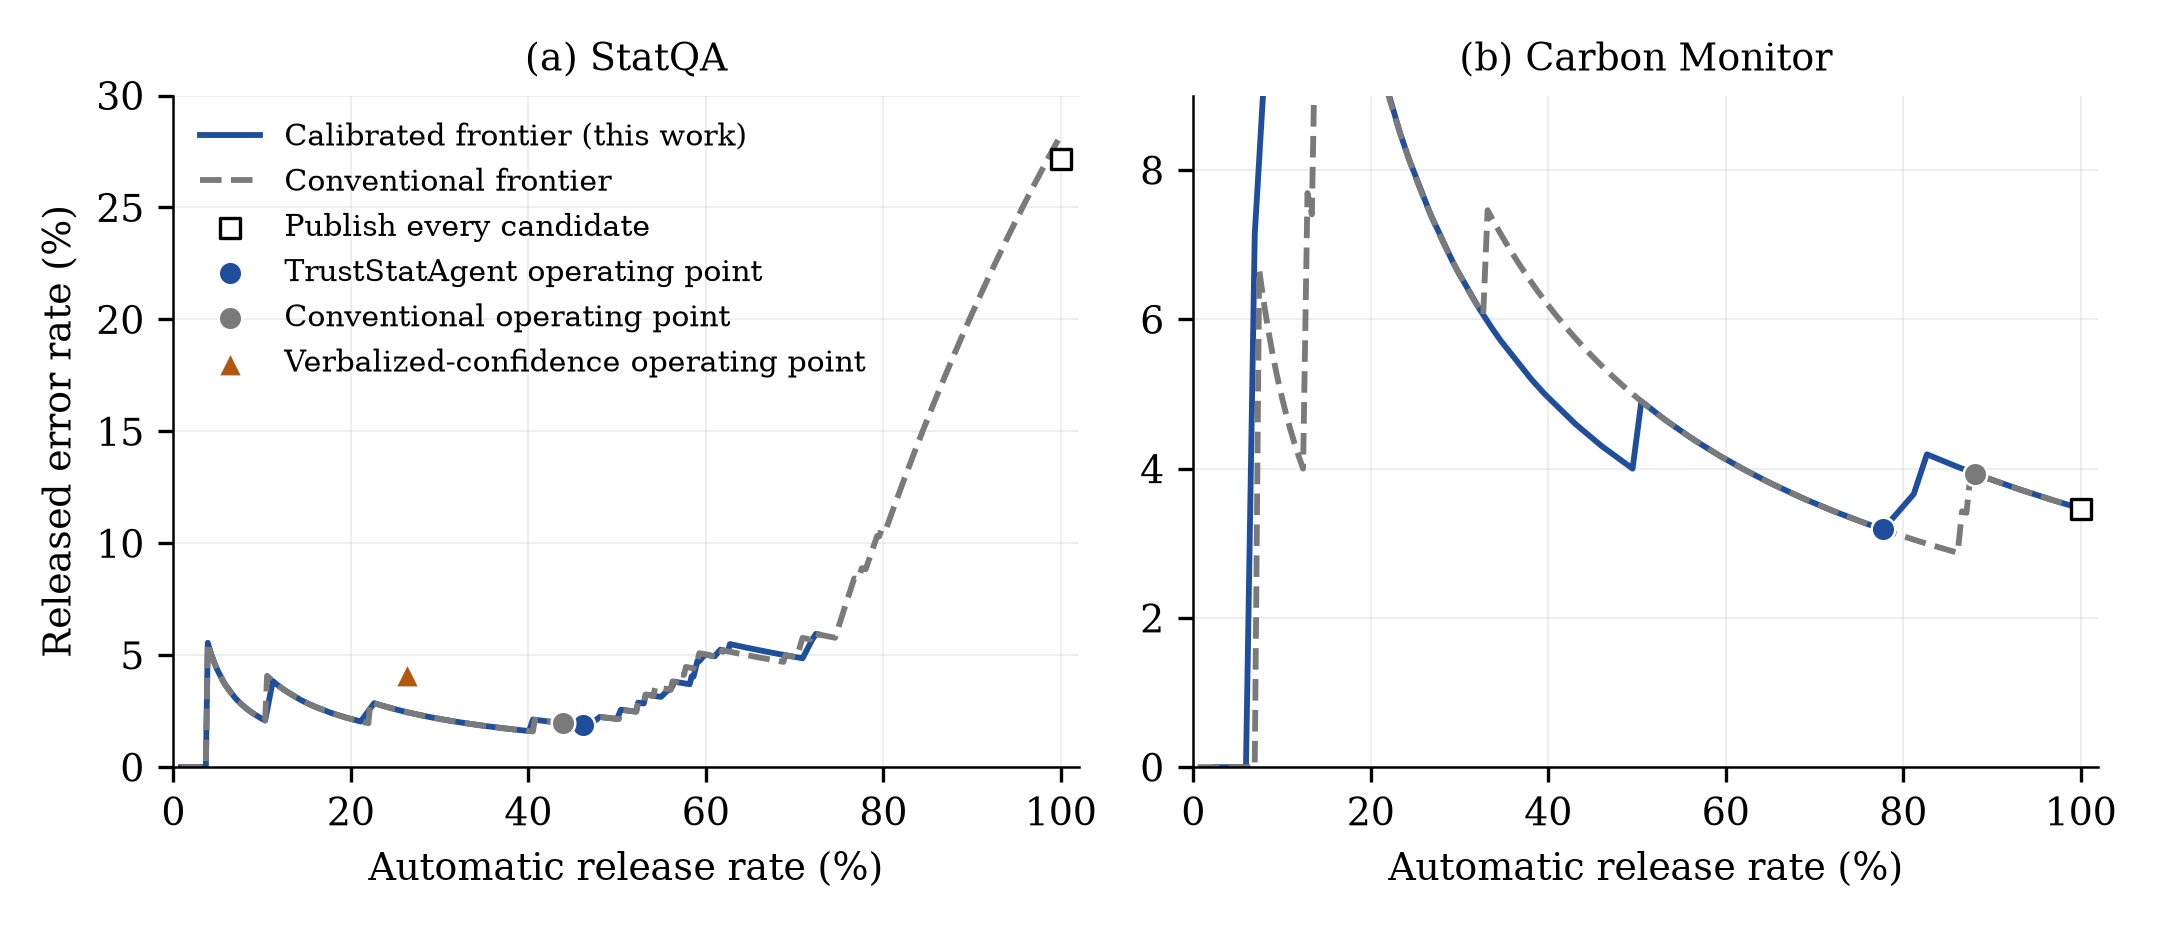
\includegraphics[width=0.8\linewidth]{figures/frontier.png}
\caption{Released error rate against release rate for the calibrated and conventional policies. Each curve is obtained by sweeping the tolerance parameter $\Delta$ with the generator, the calibration procedure, and the acceptance region held fixed. On StatQA the calibrated curve lies below the conventional one at equal release rate; on Carbon Monitor the conventional policy lies inside the frontier defined by publishing every candidate.}
\label{fig:frontier}
\end{figure}

\subsection{Limitations}
\label{sec:results_limitations}

Two assumptions carry most of the theoretical weight, and both are weaker than the experiments may suggest.
Coverage is marginal and conditional on exchangeability, which holds approximately for the tabular tasks and is explicitly not claimed for the temporal one; online conformal methods are the natural replacement for the rolling rule \citep{angelopoulos2024online}.
On StatQA the calibration units are benchmark items that differ in difficulty and in the number of admissible methods, so exchangeability across items is itself an approximation, and stratification by task type would relax it.
The bound of Eq.~\eqref{eq:release_violation_inclusion} is likewise a joint-event statement; the error rate among released results remains an empirical quantity, computed on the subset selected by the gate.

Coverage is reported as a realised quantity rather than against a target restated here.
The nominal level of each task is a configuration entry selected on the validation split, so the values of Table~\ref{tab:calibration_discrimination} are to be compared against that entry in the released configuration.
This is a reporting choice and not a weakening of the guarantee, which is stated in Section~\ref{sec:uncertainty_calibration} in terms of $\alpha$ and holds for the procedure whatever value $\alpha$ takes.

The reported figures come from a single frozen configuration.
Seed-to-seed variation of the planner, of the calibration split, and of the data partition is not quantified here, and differences of the size observed on StatQA (1.87\% against 1.96\%) and on California Housing (1.87\% against 2.02\%) would need repeated splits to establish.
The conclusions therefore rest on the larger and more consistent effects: the order-of-magnitude reduction against unrestricted publication, the lowest released error rate on all four benchmarks, and the complete failure of the conventional rule on Carbon Monitor.
The tolerance parameter $\Delta$ is prescribed rather than learned, and Fig.~\ref{fig:frontier} characterises its effect along one axis only, so a sensitivity analysis across tasks is still needed before the operating point can be recommended as a default.
Finally, the StatQA correctness scorer is a TF--IDF logistic regression frozen after training on a dedicated split (Section~\ref{sec:execution}).
This removes judge noise from the present study and means that the calibration target would have to be re-established wherever correctness is adjudicated by a different rule or by a model.

\section{Conclusion}
\label{sec:conclusion}

This paper addressed the point at which a statistical agent stops producing a result and starts publishing one.
The difficulty is not computational, since a tool can fit a model and a language model can plan which model to fit.
It is that an uncalibrated confidence score gives no finite-sample basis for deciding whether a particular result is safe to release, and that a reliability criterion taken alone can be satisfied by publishing nothing.
We therefore treated statistical accuracy and publishing reliability as a joint objective and proposed TrustStatAgent.
A tool-restricted planner produces candidates, conformal calibration attaches a coverage statement to each candidate, and a deterministic gate releases only those results whose execution is compliant and whose calibrated output lies inside the task's acceptance region.
Release authority is separated from generation, so the model that produces a number does not decide whether the number is published.

The experiments support the design on four benchmarks.
Task competence is retained, at 72.84\% official accuracy on StatQA and 84.67\% on Adult, and empirical coverage is 98.53\%, 84.23\% and 92.08\% on Adult, California Housing and Carbon Monitor.
Against publishing every candidate from the same pipeline, the gate reduces the released error rate from 27.16\% to 1.87\% on StatQA at a 46.12\% release rate and from 15.33\% to 2.72\% on Adult at 54.29\%, and it attains the lowest released error rate of the compared policies on all four benchmarks.
The ablations show that the reduction is not attributable to a single component.
Explicit planning raises candidate quality by 7.33 percentage points, removing the gate returns the released error rate to the candidate error rate, and removing calibration degrades the gate by a factor of 3.2 on StatQA and leaves it inoperative on Adult and Carbon Monitor.
The most informative result is on Carbon Monitor, where a width threshold applied to uncalibrated output withholds 11.88\% of forecasts, intercepts none of the errors, and therefore errs more among the forecasts it releases than publishing everything.
The exchange behind these figures is stated rather than concealed: where the gate costs automation it is reported as such, and the release rate accompanies every reliability figure.

Three extensions follow from these results.
First, the exchangeability assumption should be replaced by online calibration for the forecasting task and by stratified calibration for heterogeneous item pools, so that the guarantee applies to the units on which the decision is actually taken.
Second, the operating point should be derived from a stated cost ratio rather than prescribed, and the referral should distinguish degrees of review instead of the present two levels.
Third, the workflow should be tested on tasks whose correctness depends on several modelling decisions at once, such as model diagnostics and multiple-testing corrections, where the acceptance region is harder to specify than an error band but where the same separation between generation and release applies.


\bibliographystyle{elsarticle-harv}
\bibliography{references}

\end{document}
